\documentclass[times,english,12pt,twoside]{article}


\usepackage{amsmath}
\usepackage{balance}  % to better equalize the last page
%%\usepackage{graphics} % for EPS, load graphicx instead
\usepackage{graphicx}
%\usepackage{subfigure}
\usepackage[font = small]{caption}
%\usepackage{subcaption}
\usepackage{subfig}

\usepackage{txfonts}
\usepackage{color}
\usepackage{cite}
\usepackage{textcomp}
\usepackage{geometry}
\usepackage{booktabs}
\usepackage{todonotes}
\usepackage{multirow}
\usepackage{comment}
\usepackage{url}
\usepackage[linesnumbered,ruled,vlined]{algorithm2e}
\usepackage{setspace}
\geometry{verbose,a4paper,tmargin=2.54cm,bmargin=2.54cm,lmargin=3.00cm,rmargin=2.04cm}
%\usepackage[automake, acronym]{glossaries}
\usepackage{afterpage}
\usepackage{enumitem}
\usepackage{subfig}

\newcommand\blankpage{%
	\null
	\thispagestyle{empty}%
%	\addtocounter{page}{-1}%
	\newpage}

%\numberwithin{page}{section}
%\renewcommand{\thepage}{\thesection-\arabic{page}}
%\makeatletter
%\section \patchcmd{\@sect}
%{\protected@edef}
%{\def\arg{#1}\def\arg@{section}%
%    \ifx\arg\arg@\stepcounter{page}
%    \fi
%    \protected@edef}% <replace>
%{}{}% <success><failure>
%\makeatother

\newtheorem{theorem}{Theorem}[section]

\tolerance=1
\emergencystretch=\maxdimen
\hyphenpenalty=10000
\hbadness=10000

%\lefthyphenmin5
%\righthyphenmin5
%\hyphenation{op-tical net-works semi-conduc-tor}

\newcommand{\newnote}[2]{\todo[linecolor=#1,backgroundcolor=#1!25,bordercolor=#1]{#2}}
\newcommand{\snotesc}[1]{\newnote{red}{SC: #1}}
\newcommand{\snoteam}[1]{\newnote{blue}{AM: #1}}

\newcommand{\notesc}[1]{\snotesc{}\textcolor{red}{SC: #1}}
\newcommand{\noteam}[1]{\snoteam{}\textcolor{blue}{AM: #1}}

\newcommand{\blue}[1]{{#1}}
\newcommand{\red}[1]{\textcolor{red}{#1}}

\newcommand{\lastaccessedtoday}{Last accessed: \today}
\newcommand{\etal}{{\it et. al.} }

\let\oldnl\nl% Store \nl in \oldnl
\newcommand\nonl{%
	\renewcommand{\nl}{\let\nl\oldnl}}

\begin{document}
	\title{\bf{Federated Live Streaming with DASH Support}}
\date{}
\author{}
\maketitle
\thispagestyle{empty}
\begin{center}
	\vspace*{5mm}
	\textit{Extension Seminar Report Submitted in Partial}
	\par
	\vspace*{4mm}
	\textit{Fulfillment of the Requirements for the Degree of}
	\par
	\vspace*{5mm}
	{\large\textbf{Doctor of Philosophy}\\
		\vspace*{2mm}\textit{in}\\
		\vspace*{2mm}\large\textbf{Computer Science and Engineering}
		\\\vspace*{2mm}\textit{by}\\
		\vspace*{2mm}}
	\author{\large\textbf{Abhijit Mondal}\\
		\vspace*{2mm}{\small{[Roll No - 15CS91R09]}}\\
		\vspace*{15mm}\textit{Under the supervision of}\\
		\vspace*{2mm}\textbf{Dr. Sandip Chakraborty}\\}
	\vspace*{30mm}
	\begin{figure}[!ht]
		\centering
		
\includegraphics[width=3cm]{img/iit_logo}
	\end{figure}
	\bf{Computer Science and Engineering
		\\Indian Institute of Technology Kharagpur
%		\\Kharagpur - 721302, West Bengal, India
	}\\
	\date{May 24, 2019}
\end{center}
\newpage
	\blankpage
	\addtocounter{page}{-2}
%	\begin{abstract}

Adaptive bitrate video streaming over the Internet typically uses HTTP over TCP. Lately Quick UDP Internet Connection (QUIC) protocol, introduced by Google, has been shown to improve web browsing performance over TCP. Engineered to have better connection establishment, congestion control, and stream multiplexing capabilities, QUIC seems to be an obvious candidate for replacing TCP for video streaming over the web. In this work, we focus on comparing adaptive bitrate streaming performance over QUIC and TCP. Our experimental analysis is based on $175$ YouTube video streams that are accessed from a browser, and over a controlled network setup such that impact of different parameters can be studied. We observe that QUIC is better in maintaining a higher bitrate during playback, as well as, reduces bitrate switching, relative to TCP. However, QUIC uses more bandwidth to download higher data volume for buffering, especially at low bandwidth, and even suffers from more rebuffering events during playback compared to the use of TCP.

%Quick UDP Internet Connection (QUIC) is an experimental protocol developed by Google, which claims to solve the connection setup and congestion control overhead of popular Transmission Control Protocol (TCP) for large number of parallel data flows over the Internet, while providing an end-to-end secure connection. 
%The existing studies of QUIC performance show that it is good for web access as it is a light-weight protocol and can significantly reduce page download time compared to TCP. 
%However, a large number of todays' Internet traffic is based on multimedia streaming applications, such as NetFlix, YouTube and so on, and it is not known whether or how QUIC can improve the adaptive streaming performance over the web, compared to TCP. 
%In this work, we have downloaded around $175$ video clips of different types (video length, content encoding, content type) under controlled and monitored network conditions using both QUIC and TCP, and analyzed the adaptive streaming performance for both the scenarios. 
%We have observed that QUIC aggressively download high quality video segments even at low bandwidth, however it suffers from large number of re-buffering compared to TCP. 
%Further, due to quality switching during adaptive streaming, QUIC also wastes a large amount of data compared to TCP.

\end{abstract}
%	\newpage
%	\blankpage

\onehalfspacing

%\subsection{Introduction}
%\blue{
%In last section we performed analysis on the YouTube's video streaming system. Google have developed a new transport protocol 
%}


%Quick UDP Internet Connection (QUIC)~\cite{langley2017quic} has been developed and experimentally deployed over the Internet by Google to replace TCP as the transport layer protocol, while addressing the limitations of TCP for end-to-end connection managements over a wide range of applications. While majority of the global Internet traffic originates from various video streaming applications, QUIC claims to reduce the YouTube rebuffering by a margin of 18\% for desktop users and 15.3\% for mobile users~\cite{langley2017quic}. As Dynamic Adaptive Streaming over HTTP (DASH)~\cite{stockhammer2011dynamic} has been a de facto for Adaptive Bitrate Streaming (ABR) over the Internet, it would be interesting to explore how QUIC performs over various ABR techniques proposed in the recent literature in terms of end users' quality of experience (QoE).


%In DASH, the videos are divided into small segments, and every segment is encoded in multiple quality levels (bitrates). The DASH client measures the network condition and requests for a video segment with the most suited quality level based on the current network condition. The network measurement and the corresponding bitrate adaptation algorithm can be tuned in DASH, and a large number of works have been proposed in the literature to select the optimal ABR technique, such as buffer based (BOLA~\cite{Spiteri2016}), using control-theoretic approach (MPC~\cite{yin2015control}), or based on deep reinforcement learning (Pensieve~\cite{mao2017neural}). However, these existing approaches do not look into the impact of the underlying transport protocols on the video streaming QoE performance. While TCP uses multiple socket connections to download the video and the corresponding audio data, QUIC multiplexes the audio and the video streams over a single UDP socket to download the entire data from the server. 
%As the ABR techniques depend on the channel throughput estimation at the client, such protocol changes are likely to impact the streaming performance. 


%With the above context, this work evaluates and compares the performance of various ABR techniques over TCP and QUIC. We develop a testbed setup with the help of a standard DASH player from the DASH Industry Forum, where we integrate the DASH player with QUIC and use emulated network environment based on a large pool of pre-collected network traffic traces.
%With a total of $45$ hours of streaming video data, we have computed three QoE metrics -- (a) average playback bitrate, (b) total rebuffering duration, and (c) playback smoothness, while streaming over both TCP and QUIC. Our thorough experiments and observations indicate that recent ABR techniques provides better QoE over TCP compared to QUIC. We investigate further to understand the protocol-level behavior of QUIC, which impacts the QoE performance.
%Our analysis reported in this work can help the community to tweak the QUIC configurations to obtain the best QoE performance from the modern ABR techniques.
The video streaming service works at the application layer of the TCP/IP networking stack, so do the ABR algorithms. Thus these services can observe the application layer throughput only. However, application layer throughput also depends on the underlying transport protocol. For example, TCP itself has several congestion control algorithms for different scenarios. Further, there are two different transport protocols, TCP and QUIC, that are widely used nowadays for supporting video streaming applications. All these things can affect the decision of an ABR algorithm. 

To understand how QUIC works with the state-of-the-art adaptive streaming protocols, we perform a study to compare the performance of ABR algorithms on top of QUIC and TCP. To do this study, we use open source DASHIF player as it is openly available, and we can set the testbed over any platform of our choice. The detailed experimental setup follows. 

As we discussed before, any ABR algorithms' performance depends on various factors, including the underlying transport protocol. 
Recently Google has developed and experimentally deployed over the Internet a new transport protocol called \textit{Quick UDP Internet Connection} (QUIC)~\cite{langley2017quic} to replace TCP as the transport protocol, while addressing the limitations of TCP for end-to-end connection managements over a wide range of applications. While the majority of the global Internet traffic originates from various video streaming applications, QUIC claims to reduce the YouTube rebuffering by a margin of 18\% for desktop users and 15.3\% for mobile users~\cite{langley2017quic}.  It is interesting to see if that claim holds for any arbitrary ABR algorithms. We performed an analysis in a controlled environment with DASHIF players using different recently designed advanced ABR algorithms. This analysis can decide whether a new ABR algorithm is required to support video streaming for QUIC, or the old one works fine.

The performance of an ABR algorithm can indirectly impact the power consumption of smartphones due to the nature of the radio resource controller (RRC). The RRC depends on three energy state configuration. Incorrect use of radio resources can cause a lot of excess power consumption. The download pattern of the online video streaming system is bursty, i.e., sometimes it downloads data in a burst, and then it pauses for some time. The ABR algorithm decides the pause time and burst size. However, if the ABR algorithms are not aware of the RRC state, the chunk download schedule might unnecessarily consume more energy. The energy consumption by RRC depends on the signal quality as it might increase or reduce the download time of the same size segment. We perform a study using commodity smartphones to understand the relations between energy consumption and different radio signal parameters and video playback. 

%\blue{We choose DASHIF player instead of YouTube itself to control the entire testbed, which is not possible in the case of YouTube. Also, it is not possible to change the ABR algorithm on YouTube as our requirement.}

\begin{comment}
\subsection{Related Work}
Various recent studies \cite{Biswal2017,Megyesi2016} have revealed that QUIC can improve the web performance by reducing the page load time even at poor network conditions. Among them, a few works have explored the adaptive streaming performance over QUIC. In~\cite{bhat2017not}, the authors have empirically shown that DASH suffers over QUIC. Although they have given the first indication that the current ABR techniques might not perform well over QUIC, their analysis is mostly focused on buffer-based ABR and does not look into various QoE metrics as explored in the recent literature~\cite{yin2015control,mao2017neural}. In a follow-up work~\cite{bhat2018improving}, the authors have explored the QUIC retransmissions to improve the buffer-based ABR over DASH. In~\cite{van2018empirical}, the authors have used an emulated setup to analyze the buffer-based ABR techniques over QUIC and also proposed a QoE prediction mechanism for adaptive streaming over QUIC. Also, these existing studies have indicated that QUIC might not suit well for buffer-based ABR. They have not explored the performance of advanced ABR techniques over QUIC. We argue that there is a requirement to analyze the recent ABR techniques like MPC~\cite{yin2015control} and Pensieve~\cite{mao2017neural} over QUIC because these recent studies have indicated that buffer-based techniques are aggressive towards video-bitrate maximization whereas suffers in terms of playback smoothness and rebuffering. To the best of our knowledge, this is the first study that explores the performance of advanced ABR techniques over QUIC as the end-to-end transport protocol.

\end{comment}
\section{Performance Analysis of State-of-the-Art ABR Algorithms over QUIC}
\label{chap04:sec:qui-dash}
In this section, we evaluate and compare the performance of various ABR
techniques over \ac{TCP} and \ac{QUIC}. We develop a testbed setup with the help of a standard DASH player from the \ac{DASH} Industry Forum, where we integrate the \ac{DASH} player with \ac{QUIC} and use emulated network environment based on a large pool of pre-collected network traffic traces. With a total of $45$ hours of streaming video data, we have computed three \ac{QoE} metrics -- (a) average playback bitrate, (b) total rebuffering duration, and (c) playback smoothness, while streaming over both \ac{TCP} and \ac{QUIC}. The detailed experimental setup follows. 

\subsection{Experimental Setup}
\label{chap03s2:sec:experimentalSetup}
For a fair comparison between the performance of \ac{DASH} over \ac{TCP} and \ac{QUIC},
we use an experimental test network as shown in \fig\ref{fig:chap03s2:expeirmental_setup}. We use a streaming server to keep all the videos encoded at different video bitrates as mentioned later and a web-based javascript DASH player provided by \ac{DASH-IF} to stream the videos at the client side. To emulate realistic traffic behavior over the test setup, we use a benchmark traffic shaper {\tt Mahimahi}~\cite{mahimahi} and have created {\tt Mahimahi} compatible traces from two publicly available datasets -- (i) a broadband trace from FCC~\cite{dataset-fcc} and (ii) the 3G/HSDPA mobile dataset collected in Norway~\cite{dataset-norway}.

\begin{figure}[h]
	\centering
	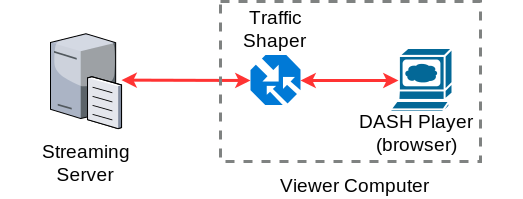
\includegraphics[width=0.8\linewidth]{img/experimental_setup}
	\caption{\label{fig:chap03s2:expeirmental_setup}Experimental setup for video streaming using DASH}
\end{figure}

We run two servers with the different end-to-end data transfer protocols, one for \ac{QUIC} and another for \ac{TCP}. For \ac{QUIC} server, we use the {\tt golang} implementation of \ac{QUIC} -- \texttt{GO-QUIC}\footnote{\url{https://github.com/lucas-clemente/quic-go} (\lastaccessedtoday)} (release version 12.0). We have also tested with other \ac{QUIC} implementations like LiteSpeed \ac{QUIC}~\footnote{\url{https://github.com/litespeedtech/lsquic} (\lastaccessedtoday)} and have similar observations as reported in this chapter. We give the results corresponding to the \texttt{GO-QUIC} implementation as it has been used by majority of the existing works in literature. For TCP based server, we use the standard {\tt webfsd}\footnote{https://www.gsp.com/cgi-bin/man.cgi?section=1\&topic=webfsd (\lastaccessedtoday)} web-server (version 1.21). As only the {\tt Google Chrome} and the {\tt Chromium} browsers support the \ac{QUIC} protocol, we use the {\tt Google Chrome} browser of compatible version 68, for our experiments to stream the videos at the client side over the \ac{DASH-IF} streaming player.


In all the experiments, we use off-the-shelf applications and run them in a non-root user mode. The streaming server and the \ac{DASH} players run over systems with 8GB of RAM and Intel(R) Core(TM) i5-4590 CPU @ 3.30GHz processor running Ubuntu 16.04.6 LTS operating system on top of Linux 4.9.78. For \ac{DASH} client, we modify dash.js v2.9.3 to add support for advance \ac{ABR} algorithms like Pensieve and MPC.


\begin{table}[h]
     \caption{\label{table:chap03s2:bitrate}Bitrate and resolution map of DASHified videos.}
	\centering
	\begin{tabular}{|l|c|c|c|c|}
		\hline
		Bitrate(kbps) & 200 & 400 & 600 & 800 \\ \hline
		Resolution & 320x180 & 320x180 & 480x270 & 640x360 \\ \hline \hline
		Bitrate(kbps) & 1000 & 1500 & 2500 & 4000 \\ \hline
		Resolution & 640x360 & 768x432 & 1024x576 & 1280x720 \\ \hline
	\end{tabular}
\end{table}

We use a total of $45$ hours of videos (about $57$ different videos) which have been dashified (encoded in different bitrates as shown in \tbl\ref{table:chap03s2:bitrate}) using the {\tt ffmpeg} tool in eight different video quality levels and two different audio quality levels. We play every videos for all the \ac{ABR} algorithms and protocol combinations, resulting $\approx 19$ days of video playback time. We also maintain the similar playback environment for DASH/QUIC and DASH/TCP for each of the video and the \ac{ABR} combinations. 
We have compared the performance across five different \ac{ABR} mechanisms, namely, BOLA (B)~\cite{Spiteri2016}, the standard buffer-based quality adaptation of \ac{DASH-IF} (BB), the two variants of MPC driven approaches~\cite{yin2015control} -- MPC-Fast (MF) and MPC-Robust (MR) and the deep learning driven quality adaptation algorithm -- Pensieve (P)~\cite{mao2017neural}. To measure the overall \ac{QoE} of the video playback, we have used a combined metric of the average quality level, the rebuffering time and the playback smoothness, as used in~\cite{yin2015control,mao2017neural}.
\begin{equation}
QoE=\sum_{i=1}^{N}q(R_i)-\mu\sum_{i=1}^{N}\delta_i-\sum_{i=1}^{N-1} \bigg\vert q(R_{i+1})-q(R_i)  \bigg\vert
\label{eqn:chap03s2:QoE}
\end{equation}
We modify \eqn\ref{eqn:QoE} as \eqn\ref{eqn:chap03s2:QoE}, which indicates the \ac{QoE} metric to measure the overall \ac{QoE} of a video playback session. Here, $N$ is the total number of chunks for the playback video. $R_i$ and $q(R_i)$ are the representation of the playback bitrate of the chunk $i$ and the quality perceived by a user for that chunk $i$. $\delta_n$ is the rebuffering time for the chunk $i$. $\mu$ is a QoE weight factor \cite{yin2015control}.
We consider a linear representation $q(R_n) = R_n$, similar to~\cite{yin2015control}, indicating that the playback quality increases linearly with the increase of playback bitrate.

\begin{figure*}[!t]
	\begin{minipage}[t]{0.48\linewidth}
		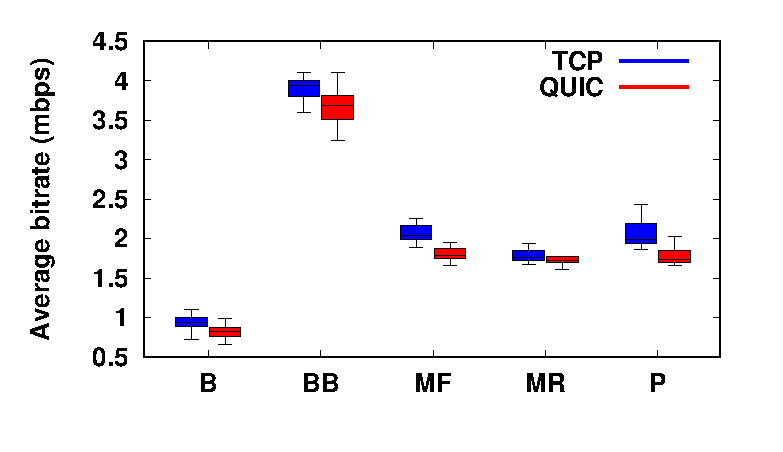
\includegraphics[width=\linewidth]{img/newexp/bitrate_box}
		\caption{\label{fig:chap03s2:averageQuality_n}Average Playback Video Quality for Different ABR Techniques ($p<0.05$ for all the metrics)}
	\end{minipage}\hfill
	\begin{minipage}[t]{0.48\linewidth}
		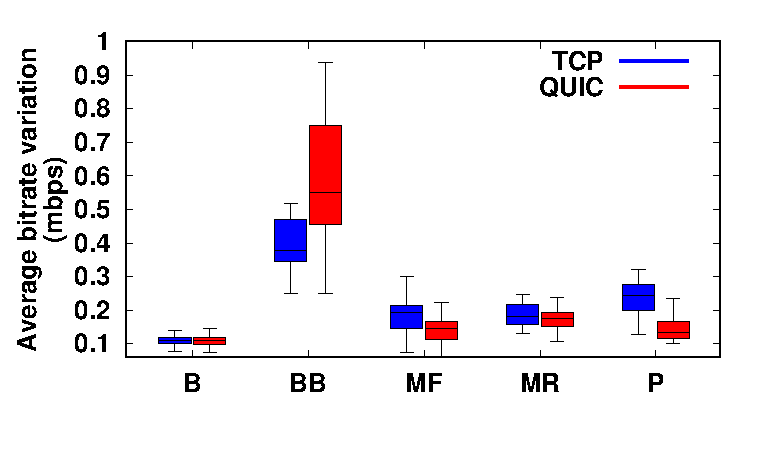
\includegraphics[width=\linewidth]{img/newexp/smooth_box}
		\caption{\label{fig:chap03s2:averageQualityVariation_n}Average Playback Quality Variation for Different ABR Techniques ($p<0.05$ for all the metrics except BOLA and MPC-Robust)}
	\end{minipage}

	\begin{minipage}[t]{0.48\linewidth}
		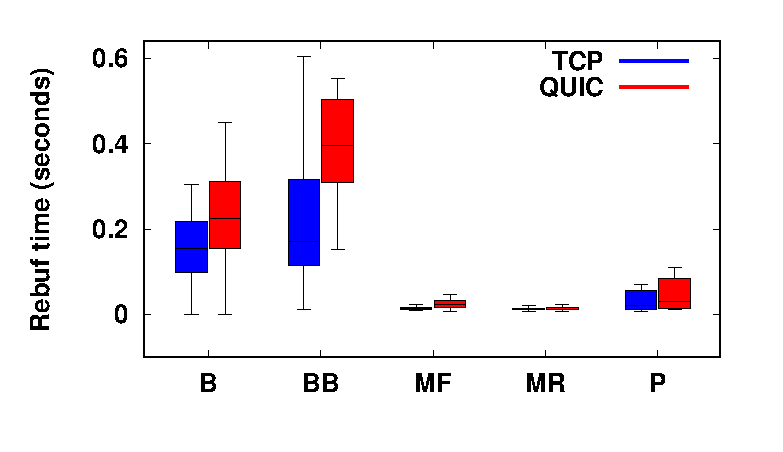
\includegraphics[width=\linewidth]{img/newexp/rebuf_box}
		\caption{\label{fig:chap03s2:RebufferTime_n}Rebuffering Time for Different ABR Techniques ($p<0.05$ for all the metrics except Pensieve and MPC-Robust)}
	\end{minipage}\hfill
	\begin{minipage}[t]{0.48\linewidth}
		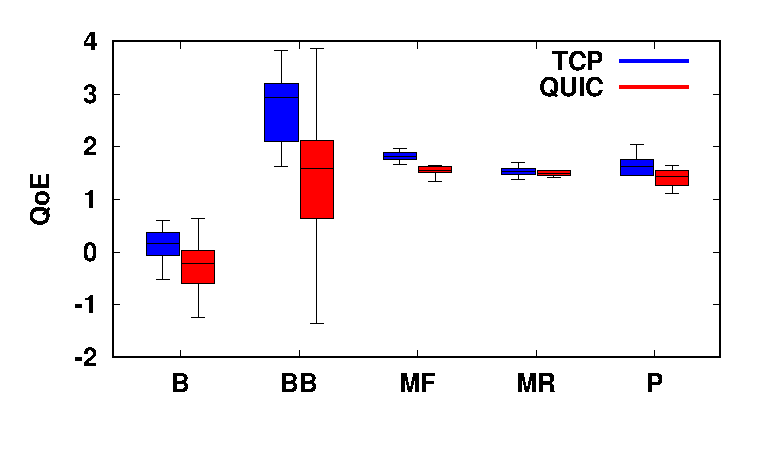
\includegraphics[width=\linewidth]{img/newexp/qoe_box}
		\caption{\label{fig:chap03s2:QOE_n}Overall QoE for Different ABR Techniques ($p<0.05$ for all the metrics except MPC-Robust)}
	\end{minipage}
\end{figure*}

\subsection{Results and Analysis}
We first look into the overall playback video quality and then dig into the details of individual QoE metrics. As the data used for this analysis have been collected from realistic experiments, we, therefore, avoid any underlying parametric assumption while checking for the statistical significance of the results. Subsequently, we apply Mann–Whitney U test~\cite{mannwhitney} with non-parametric assumptions on all the metrics and report if the results are statistically significant or not with the hypothesis that DASH/TCP works significantly better than DASH/QUIC\footnote{We use the notation ``DASH/TCP'' to indicate DASH over TCP; similarly ``DASH/QUIC'' indicates DASH over QUIC.}. We also run a two-way test to check the alternate hypothesis that DASH/QUIC works significantly better than DASH/TCP.




\subsubsection{Average Video Bitrate}
The distributions of the average playback bitrate for the five ABR mechanisms are shown in Fig.~\ref{fig:chap03s2:averageQuality_n}. For BOLA, we observe that the average video bitrate for DASH/TCP is higher than that of DASH/QUIC. It is known from the existing literature that buffer-based ABR mechanisms aggressively use the highest quality levels, which we also observe in Fig.~\ref{fig:chap03s2:averageQuality_n}. However, we observe that DASH/TCP always performs better than DASH/QUIC. Indeed, the state-of-the-art reinforcement learning based ABR mechanism, Pensieve, provides much better quality level on top of TCP in comparison to QUIC. For all the five ABR methods, we observe that the $p$-value is less than $0.05$ for the Mann–Whitney U test, indicating that DASH/TCP performs significantly better than DASH/QUIC in terms of average playback quality.

\subsubsection{Quality Level Fluctuation -- Playback Smoothness}
Next, we observe the average fluctuation in the playback quality levels, which has been shown in Fig.~\ref{fig:chap03s2:averageQualityVariation_n}. A fluctuation in the quality level indicates less smoothness in the video playback, and, therefore, reduces the QoE. We observe that the differences in average quality level fluctuations between DASH/TCP and DASH/QUIC for BOLA and MPC-Robust are statistically insignificant. However, the figure indicates that quality fluctuation with DASH/QUIC is significantly more for buffer-based ABR, whereas less for MPC-Fast and Pensieve-based ABR, with $p$-value less than $0.05$. This is an interesting observation as we see that the advanced ABR techniques, such as MPC-Fast and Pensieve, provide better playback smoothness with DASH/QUIC, although the supported playback quality is lower compared to DASH/TCP. 


\subsubsection{Rebuffering Time}
Fig.~\ref{fig:chap03s2:RebufferTime_n} indicates the rebuffering time for different ABR techniques over DASH/TCP and DASH/QUIC. We observe that rebuffering is significantly more with DASH/QUIC for BOLA, buffer-based and MPC-Fast, whereas the differences in rebuffering are statistically insignificant for MPC-Robust and Pensieve. For the buffer-based ABR which aggressively download the videos at the highest playback quality, rebuffering is comparatively very high with DASH/QUIC. MPC-Robust and Pensieve show minimal rebuffering, so the differences between DASH/TCP and DASH/QUIC are not statistically significant. We observe that the claim from Google~\cite{langley2017quic} that QUIC enables less rebuffering does not hold for all the ABR techniques and is very much specific to which ABR technique is adopted at the playback client.  


\subsubsection{Overall QoE}
Finally, we look into the overall QoE computation as shown in Eq.~(\ref{eqn:chap03s2:QoE}). The overall QoE measurements for  all the ABR techniques are shown in Fig.~\ref{fig:chap03s2:QOE_n}. In this experiment, we plot the linear variants of $q(R_n)$ as discussed in the previous section. Our observations from these results are as follows. DASH/TCP provides significantly better QoE compared to DASH/QUIC for all the ABR algorithms except MPC-Robust where the result is statistically insignificant. This indicates that the recent advanced ABR techniques like MPC and Pensieve are more compatible with TCP than QUIC. Indeed from representations of $q(R_n)$, we can say that the above observations are generic across a wide variation of QoE measurements. 



\subsection{Looking Under the Hood}
Our thorough experiments over a wide range of ABR techniques indicate that DASH over QUIC does not perform as well as it is supposed to. To explore this further, we perform a set of experiments to understand the issues with QUIC, which affect DASH-based video streaming.

\subsubsection{Does QUIC Perform Poorly in All Scenarios?}
One immediate question that might arise in this context is whether the observed performance drops are generic for QUIC, or whether certain features of QUIC affect the performance of DASH. With the similar network setup as discussed before, we compute the overall throughput and the response latency for TCP and QUIC over two different scenarios -- (a) downloading of large web-objects and (b) DASH video streaming.

\newcommand{\subsubsubsection}[1]{\textbf{#1: }}
\subsubsubsection{Performance during HTTP Object Downloads}
To see how the performances of TCP and QUIC fare during the download of HTTP web objects, we perform a set of experiments over the same network setup with emulated bandwidth control via {\tt Mahimahi} traffic shaper. We download HTTP web objects (HTML and data files) of predefined sizes (from $2$MB to $50$MB) for $40$ sequential HTTP requests in each session. We give a pause of $500$ms before requesting the next web object. We repeat each session three times for both TCP and QUIC. 


\begin{figure}[!ht]
	\captionsetup[subfigure]{}
	\begin{center}
		\subfloat[\label{fig:chap03s2:proofLargeFileThroughput}Throughput]{
			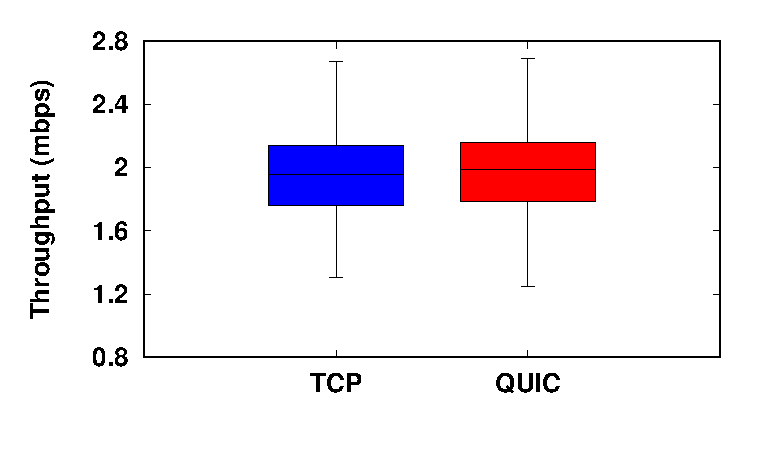
\includegraphics[width=.49\linewidth]{img/proof/largefile/throughput}
		}
		\subfloat[\label{fig:chap03s2:proofLargeFileWait}Response latency]{
			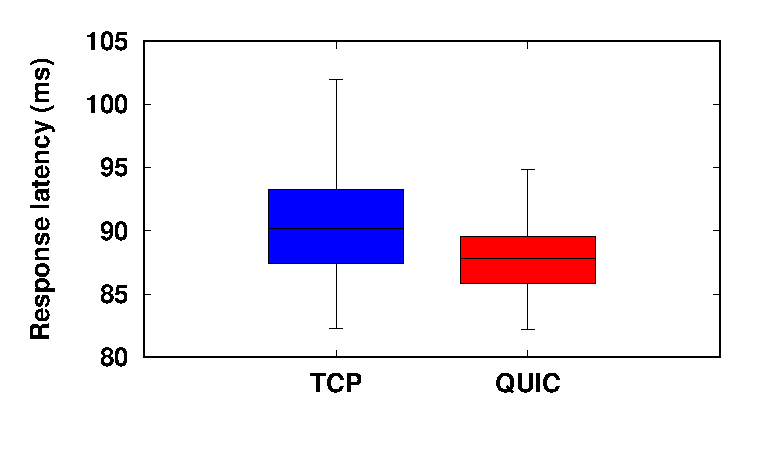
\includegraphics[width=.49\linewidth]{img/proof/largefile/wait}
		}
	\end{center}
	\caption{\label{fig:chap03s2:proofLargeFile}TCP and QUIC performance during HTTP web object download}
\end{figure}


\fig\ref{fig:chap03s2:proofLargeFileThroughput} shows the distribution of throughput observed against each web object downloads, while \fig\ref{fig:chap03s2:proofLargeFileWait} indicates the response latency observed by each HTTP request. The throughput is computed as the object size divided by the download time where the download time is the time difference between the first and the last bytes received for that web object. The response latency is computed as the time between the initiation of the HTTP request and the time when the first byte of the response is received. From the figures, we see that the throughput is similar for HTTP/TCP and HTTP/QUIC. The response latency for HTTP/QUIC is slightly lower than HTTP/TCP. These experiments shows that QUIC performs better than TCP in terms of response latency which is an important QoE metric for web object downloads. 


\begin{figure}[!ht]
	\captionsetup[subfigure]{}
	\begin{center}
		\subfloat[\label{fig:chap03s2:proofCompThroughput} Throughput ]{
			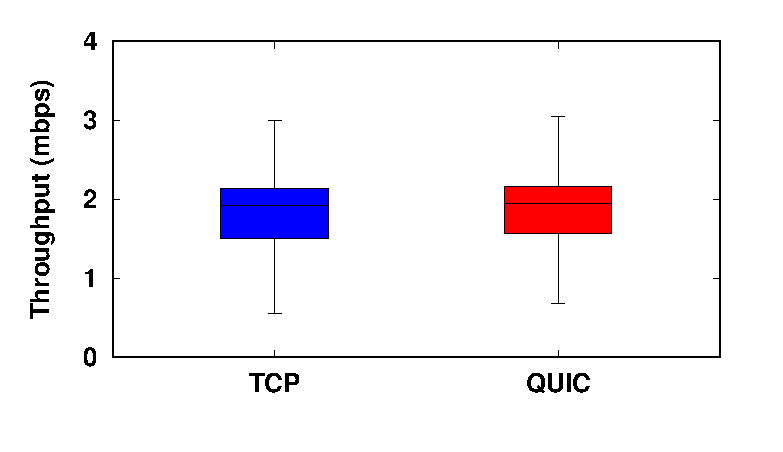
\includegraphics[width=.45\linewidth]{img/proof/comp/throughput}
		}
		\hfill
		\subfloat[\label{fig:chap03s2:proofCompWait} Response latency]{
			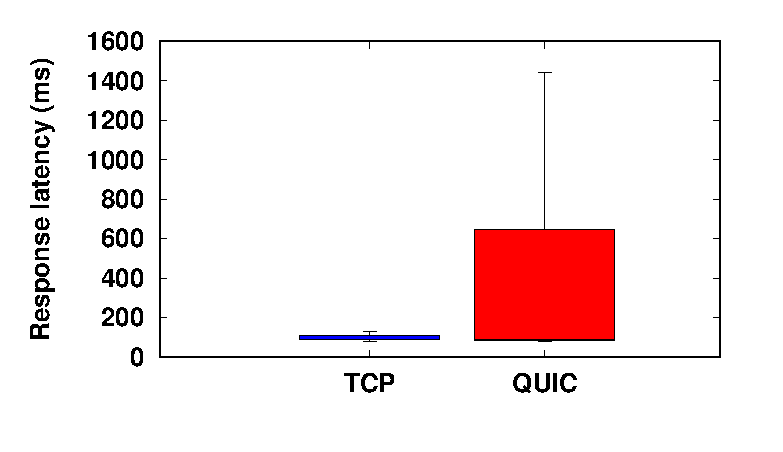
\includegraphics[width=.45\linewidth]{img/proof/comp/wait}
		}
	\end{center}
	\caption{\label{fig:chap03s2:dashcomp}TCP and QUIC performance during DASH video segment download}
\end{figure}


\subsubsubsection{Performance during Video Streaming}
\fig\ref{fig:chap03s2:proofCompThroughput} shows the distribution of the throughput observed during the video playback, combining the data from all the five ABR mechanisms. A statistical test also indicates that the difference between TCP and QUIC in terms of throughput is not significant. Interestingly, the predicted throughput during video streaming is one of the important metrics used by all the ABR mechanisms for deciding the optimal bitrate. \fig\ref{fig:chap03s2:proofCompWait} plots the distributions of the response latency, combining the videos from all the five ABR mechanisms. We have an interesting observation here -- although the difference in the median of the response latency for DASH/QUIC and DASH/TCP is not significant,  the upper quartile for the response latency of DASH/QUIC is significantly higher than the upper quartile of DASH/TCP. This indicates that with QUIC, the response latency sometime becomes very high -- this observation is opposite to what we have observed in \fig\ref{fig:chap03s2:proofLargeFileWait}. It can be noted that the throughput computation does not consider the response latency, rather it considers the time difference between the first and the last bytes received for a video segment. The ABR algorithms primarily select the bitrate based on the computed throughput for the last few video segments. If the computed throughput is high, the DASH client requests for the next video segment in an increased quality level. However, if the response latency is high, this segment may take longer time to reach the client, resulting in a rebuffering and subsequent drop in the quality levels for the next video segments. We do not see this problem for TCP, as the response latency correlates with the computed throughput; however, this correlation does not hold for QUIC. Next, we dig further to find out the reason behind the high response latency observed during the video streaming using QUIC.

\subsubsection{Exploring TCP and QUIC Connections during a Video Streaming}
During the dashification of a video with an embedded audio, the standard practice is to first segregate and segment the video data and the corresponding audio data, and then encode the video and the audio segments separately in their respective available encoding formats.
Now the DASH client creates two different HTTP streams for downloading the video segments and the corresponding audio segments. For DASH/TCP, two different TCP sockets are created between the DASH client and the server for these two HTTP streams, whereas for DASH/QUIC, both the HTTP streams are multiplexed, and the HTTP messages are exchanged over a single UDP socket.
This brings the next question -- how do TCP and QUIC fare for two parallel but interdependent application streams between the same client and the server?  To answer this question, we do the next experiment over the same network setup as discussed before. In this experiment, we create two HTTP streams where both the streams request for the HTTP objects (files) in parallel. The object sizes are varied from $1$MB to $8$MB.
We also vary the duration between two HTTP requests (called the pause time) from $500$ms to $8000$ms. 

\begin{figure}[!ht]
	\captionsetup[subfigure]{}
	\begin{center}
		\subfloat[\label{fig:chap03s2:proofUhoodMThroughput2} Throughput]{
			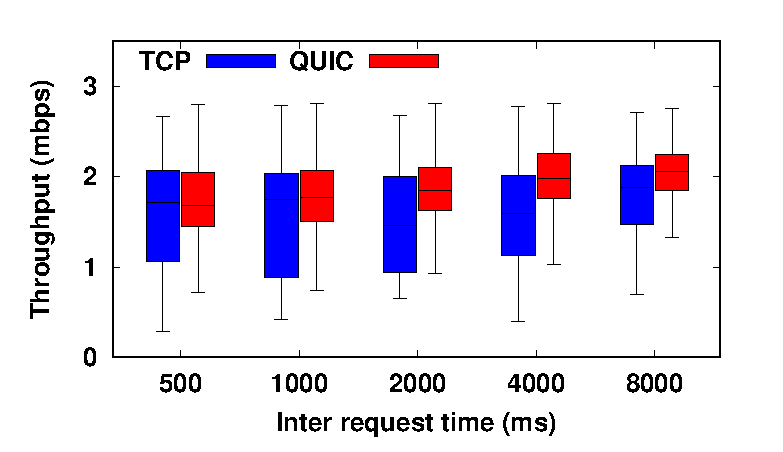
\includegraphics[width=.49\linewidth]{img/proof/uhoodM/throughput-2}
		}
		\subfloat[\label{fig:chap03s2:proofUhoodMWait2} Response latency ($p<0.05$ for all the instances)]{
			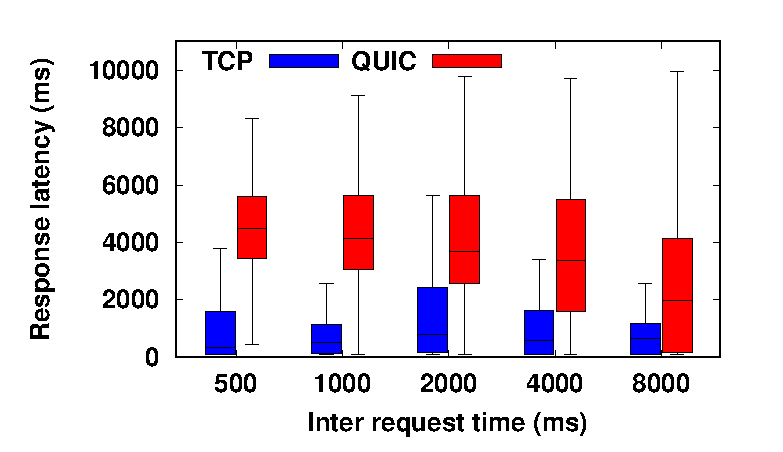
\includegraphics[width=.49\linewidth]{img/proof/uhoodM/wait-2}
		}
	\end{center}
	\caption{\label{fig:chap03s2:proofUhoodM}Performance of TCP and QUIC for two parallel connections}
\end{figure}


\fig\ref{fig:chap03s2:proofUhoodM} shows the observations from this experiment. The differences in throughput between QUIC and TCP is not significant; however, the response latency with QUIC is significantly higher than TCP when two parallel application streams generate HTTP requests. Further, this difference in the response latency is more prominent when the pause time is less indicating the frequency of the HTTP requests is high. This observation is very synonymous to what we observed in \fig\ref{fig:chap03s2:dashcomp}. To find out the reason for such a behavior, we see that the problem is inherited from the behavior of the socket buffers used to interface between the user-space and the kernel-space. As TCP creates two separate sockets for the two HTTP streams, each of the sockets maintains its own socket buffer. Therefore, the HTTP responses from the two streams do not interfere with each other. On the other hand, QUIC multiplexes both the streams and uses a single UDP socket having a single socket buffer. Therefore, the HTTP responses from both the streams interfere, and higher response rate at one stream affects the queuing delay for the response at the other stream. 


When DASH uses two separate HTTP streams for video and audio downloads, the stream corresponding to the video downloads has a higher data generation rate compared to the stream corresponding to the audio download. This is because the amount of video data to be downloaded is much higher compared to the amount of the audio data to be downloaded, for a fixed playback time. For DASH/TCP, the audio and the video streams use separate socket buffers, having independent queuing delay depending on their data generation rate. However, for QUIC, both the streams get multiplexed. For every playback segment, the client generates one HTTP request for the video segment and another HTTP request for the audio segment. As the video segment request is sent first, the UDP socket buffer gets filled up with the majority of the video segment data. Consequently, the data for the audio segment needs to wait until that video data gets freed up from the socket buffer. \fig\ref{fig:chap03s2:proofCompDlTime} shows an example instance of video download using QUIC, where we see that video data is served almost immediately after the request is received at the server. However, the audio data has to wait in the queue (the red timeline) before it gets served. This problem is not there in TCP as the fairness property of TCP flow and congestion control serves both the socket buffers in a fair way. So, the audio data does not experience this high response latency. \fig\ref{fig:chap03s2:proofCompAVLatency} shows the distributions of the response latency for the audio and video streams separately. We see that the distributions of the response latency for the video streams are similar for QUIC and TCP. However, the audio streams at QUIC experiences a much higher latency compared to TCP. 


\begin{figure}[!ht]
	\captionsetup[subfigure]{}
	\begin{center}
   		\subfloat[\label{fig:chap03s2:proofCompDlTime} Video/Audio downloads over QUIC]{
   			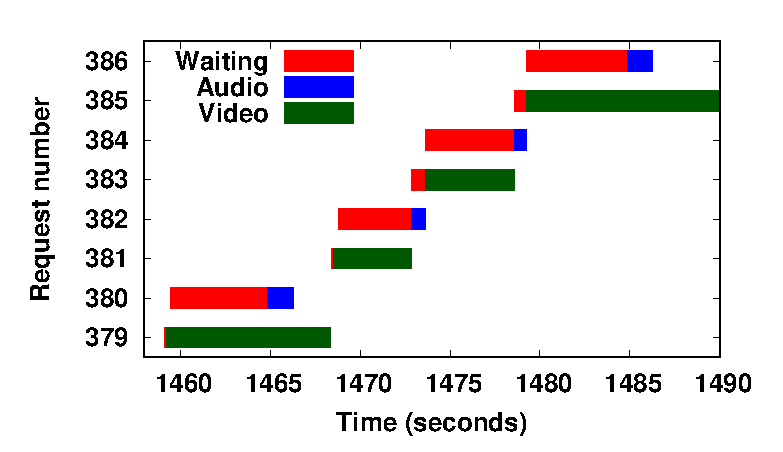
\includegraphics[width=.45\linewidth]{img/proof/comp/ls}
   		}
           		\hfill
		\subfloat[\label{fig:chap03s2:proofCompAVLatency} Response latency for audio and video]{
			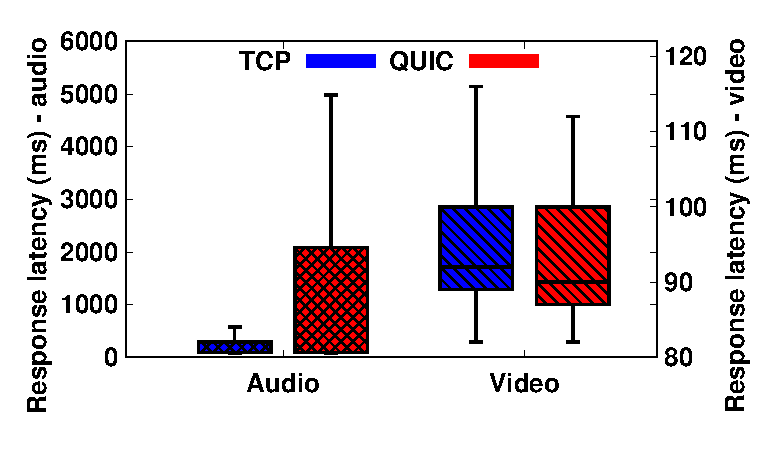
\includegraphics[width=.45\linewidth]{img/proof/comp/avwait}
		}
	\end{center}
	\label{fig:chap03s2:dashcompres}
	\caption{TCP and QUIC response latency during video and audio downloads over separate streams}
\end{figure}


\subsection{Summary}
We observe that during parallel downloads of audio and video streams, QUIC multiplexing affects the response latency of the audio streams. This observation also tallies with the observation made in~\cite{kakhki2019taking}, which states that multiplexing objects from parallel streams affect the latency of individual objects. This latency is inevitable because of multiplexing multiple objects over a single UDP queue, whereas the final video playback depends on the successful download of both the video and the audio segments. Interestingly, the throughput calculation used in DASH does not consider this response latency, resulting in a mismatch between the expected throughput and the actual download time of the segments after a request is sent. There might not be a direct solution to this problem as DASH is unaware of such behaviors of the underlying data transmission protocol, whereas QUIC is unaware of the dependency between the audio and the video streams for successful streaming of the video. We might need further investigation of the QUIC protocol stack to make it compatible with the state-of-the-art ABR streaming mechanisms.  

Apart from the protocol choices, mobility plays another important role during video streaming over smartphones. Till now, we considered the network bandwidth as the only factor for video streaming; however, as video streaming is a network-intensive application, and peoples across the globe use video streaming applications widely over smartphones, energy consumption becomes another concern. Therefore, in the next section, we investigate how video streaming applications impact the device's energy consumption due to their network-intensive activities.  





\section{Conclusion}
This letter gives an analysis of the recent advanced ABR techniques over the QUIC as the end-to-end transport protocol. We observed that all the ABR techniques are sensitive to sudden increase or drop in the client-perceived link bandwidth, and therefore are more compatible with TCP rather than QUIC. The QUIC multiplexing of audio and video streams over a single UDP socket results in additional response latency for the audio segments, which are not captured during the calculation of channel throughput. As a consequence, the ABR algorithms take incorrect decisions during selecting the bitrates based on the calculated throughput over a QUIC connection. The analysis discussed in this letter opens up a new direction of research on exploring ABR techniques over QUIC which is the de-factor transport protocol for Google services. 

%%\section{Introduction}
%During the last decade, social video streaming for targeted audiences have seen a huge boom with applications like Twitch.tv, Periscope, Meerkat along with the traditional YouTube \& Facebook live and similar other personalized live streaming services~\cite{wang2016anatomy}. Live broadcasts over such platforms have increased many-folds during the recent COVID-19 pandemic due to over-the-top (OTT) services like online live broadcast of classroom lectures to the students\footnote{\url{https://www.nokia.com/blog/network-traffic-insights-time-covid-19-march-23-29-update/} (Accessed: \today)}. Many existing studies indicate that live streaming of popular events, such as a live cricket or football match, creates multiple traffic bottlenecks in the network, particularly at the Internet gateways of private organizational networks or Internet Service Providers (ISP)~\cite{yan2018understanding}. Consequently, a question arises -- how can we prevent traffic bottlenecks in the Internet while allowing high definition video streaming to millions of users? 

In the previous chapters, we have analyzed the online video streaming systems and developed a way to reduce the energy consumption while streaming online videos. In this chapter, we consider a class of live but non-interactive streaming applications, where the video is broadcast to a set of targeted audiences over social streaming applications. Social streaming applications many-a-times form communities which are localized, forming one or more geographical clusters~\cite{wang2016anatomy}. We utilize this localized community formations among live streaming viewers to construct one or more playback coalitions, as shown in \fig\ref{fig:chap06:flsd}. The coalition members share a common network gateway (such as an organizational local network gateway or the service gateway for a cellular core network) to connect to the Internet, however, there are direct high-speed local connections among the coalition members (like \acr{LAN} connections or cellular device-to-device connections). It can be noted that such a coalition can be formed based on the principles of \ac{ALTO}, where an \ac{ALTO} server can provide the locality information of video players without requiring any explicit network or device firmware change. The coalition members collectively download the video from the content provider based on an \ac{ABR} streaming strategy, such as \ac{DASH}. The clients in a coalition collectively decide the adaptive playback rate and share data-download loads among themselves maintaining the playback synchronization. 
\begin{figure}[!ht]
    \centering
    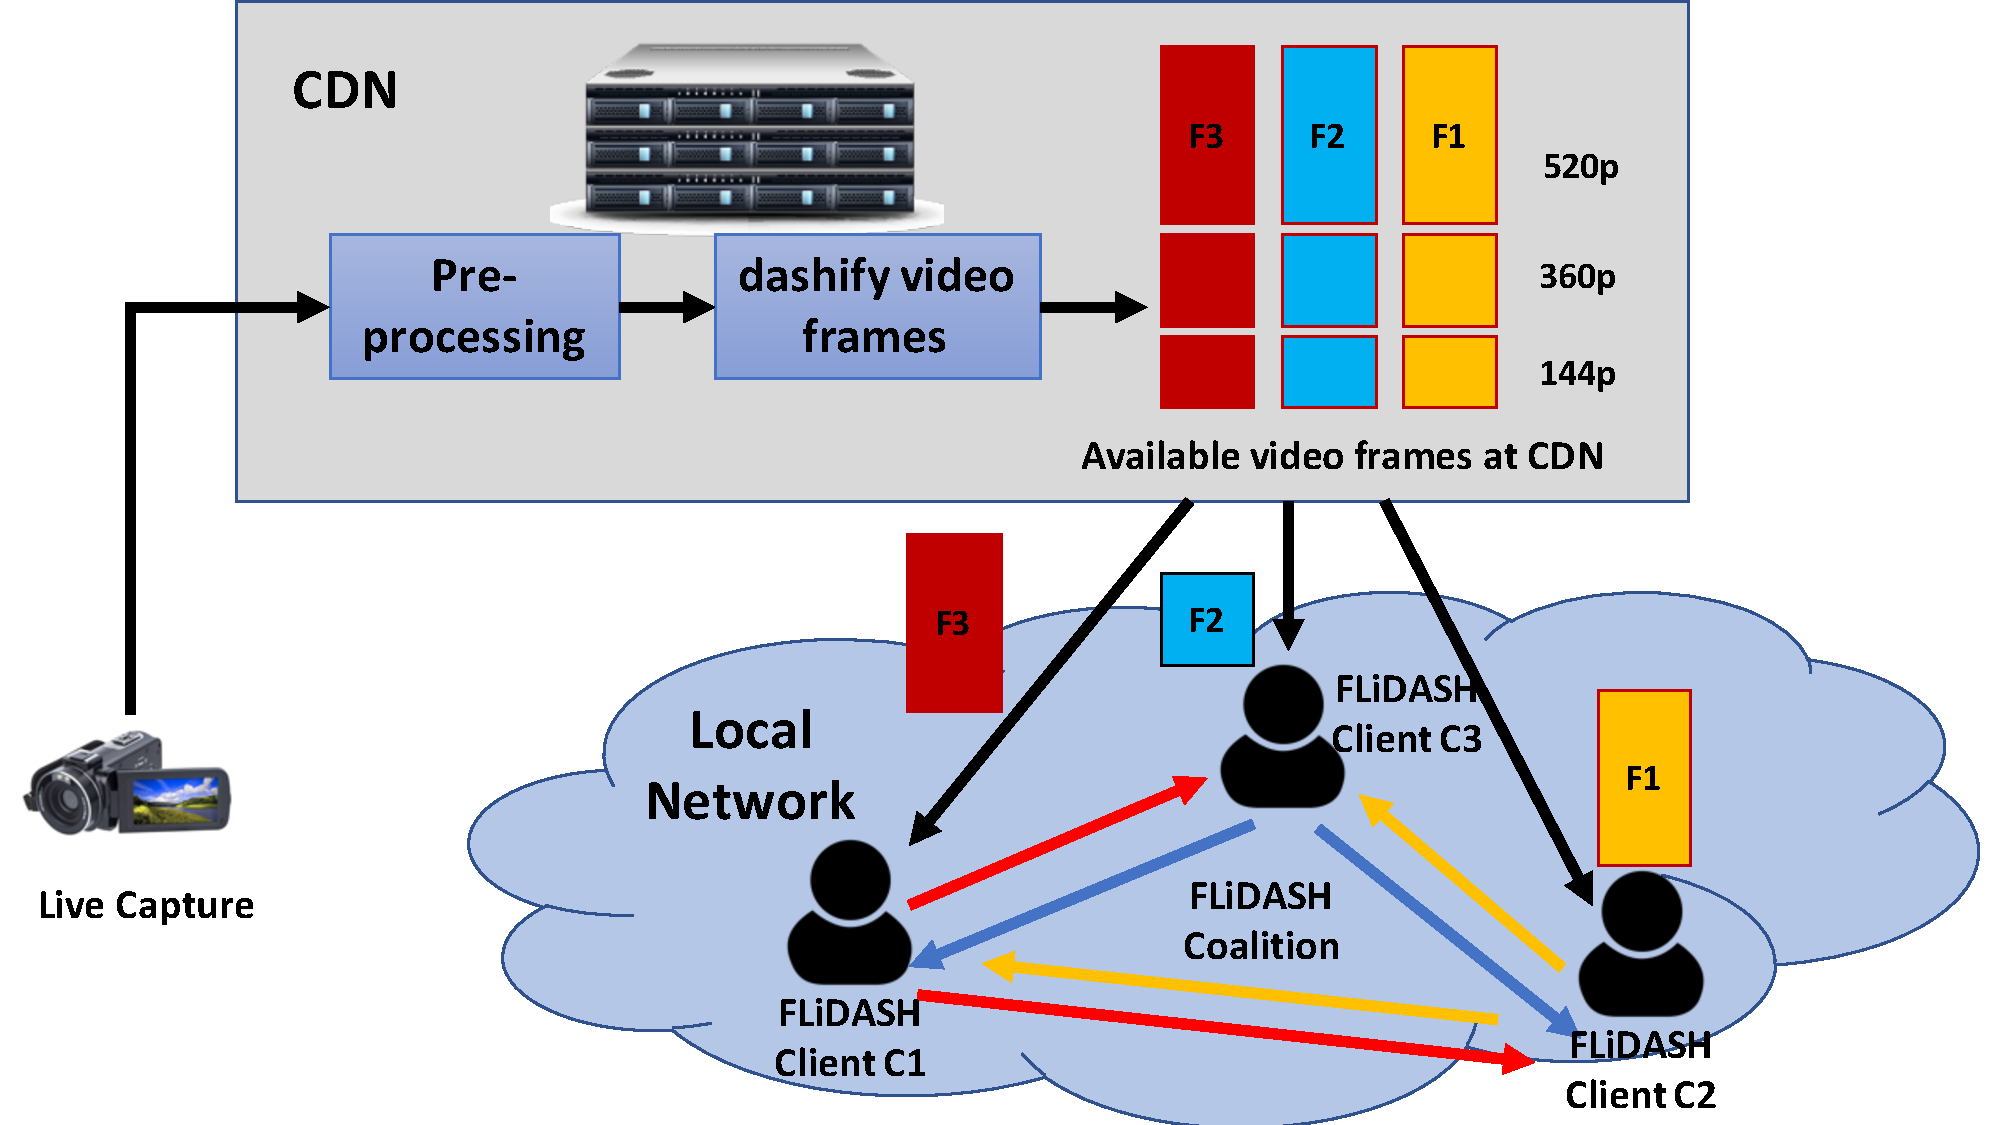
\includegraphics[width=0.8\linewidth]{img/flsd.pdf}
    \caption{Overview of \our: The clients under a local network create a coalition, every members of the coalition share the total download load.}
    \label{fig:chap06:flsd}
\end{figure}

However, developing such a system has multiple challenges. First, the coalition needs to be designed in a way such that downloading data directly from the content provider is costlier than sharing the data over the local network. Second, there should be a proper distribution of segment-wise data-download scheduling among the coalition members such that playback synchronization is not violated. A proper playback synchronization ensures that every player in the coalition should acquire the video segment $s_{i}$, either downloaded by itself or fetched from another coalition player through the direct local link, by the time it completes playing the previous video segment $s_{i-1}$; otherwise, there might be a rebuffering delay affecting the \ac{QoE}. Third, the Internet bandwidth of individual players may vary over time; therefore, the coalition as a whole should schedule the video segment downloads among its members as well as decide the bitrate of every video segment based on the \ac{ABR} principle.

Owing to the above challenges, we develop a coalition-based adaptive live streaming  called \textit{Federated Live Streaming over \ac{DASH}} (\our) where the streaming clients or players form a dynamic coalition based on the network quality parameters and collectively stream a live video. We use the playback buffer statistics at individual streaming clients to develop a distributed mechanism for coalition formation with the help from a proximity server (which can be an \ac{ALTO} server). The members of a coalition use a low-overhead gossip-based protocol for playback synchronization and takes following two decisions -- (1) scheduling the downloads of video segments among the coalition members based on their individual instantaneous network condition and the overall fairness criteria, and (2) bitrate of each video segments to optimize the overall \ac{QoE} of the coalition. We use the following \ac{QoE} objectives while making the above decisions -- (a) improve the overall video quality level, (b) improve the playback smoothness by reducing the quality fluctuations, (c) reduce rebuffering, and (d) improve fairness  among the coalition members in terms of the downloaded data share. We have implemented {\our} over an emulated environment and have thoroughly compared its performance with various other baselines. We observe that {\our} improves the overall \ac{QoE} with less traffic overhead at the backbone network.

The rest of the chapter is organized as follows. 

%
%\section{Related Work}
Various existing researches have focused on improving QoE of the ABR protocols used in DASH. Huang \etal proposed a buffer-based adaptation algorithm~\cite{buffer-based-sigcomm-2014} which has been extended later based on different approaches such as playback buffer monitoring (BOLA~\cite{Spiteri2016}), control theory (MPC~\cite{yin2015control}), reinforcement learning (Pensieve~\cite{Pensieve}), etc. Many existing literature have developed approaches to apply such ABR techniques over a live streaming platform~\cite{TNET-Migration-2016,bruneau2018pms,spiteri2019theory}, although in a pure client-server setting. 

Collaborative live streaming has been studied extensively in the literature during the last decade~\cite{jahed2016scalable,le2016microcast,Roverso:2015,saleh2016performance,khalid2019sdn}, which primarily use three different techniques. First, researchers have explored collective live streaming over a P2P setting~\cite{saleh2016performance,Collaborative-P2P-WCNC-2018}. These group of works have used a P2P network for sharing the live videos among themselves. One of the peers fetches the content from the CDN and distributes it to other peers in the network. Majority of these works use a single P2P overlay across the entire network, where the users can join or leave dynamically.  Among these works, \textit{SmoothCache 2.0}~\cite{Roverso:2015} is the closest to our architecture, where the overlay network is constructed based on a tiered-hierarchy with bandwidth-ordered fashion. The peers having the maximum bandwidth fetches the data directly from the CDN, and then the video is distributed across the lower-tiered peers. For video bit-rate adaptation, \textit{SmoothCache 2.0} keeps the first-tier for every available bit rate. We argue that this architecture places substantial overhead on the peer clients due to the complexity of overlay management. 

In contrast to this peer-to-peer overlay architecture, we consider a federated architecture, where multiple independent coalitions among the streaming clients can evolve in the network depending on the organizational network cluster. Each coalition independently and dynamically decides the video bit-rates based on the available bandwidth. The second group of works on collaborative live streaming uses cloud or SDN-assisted approaches~\cite{payberah2012clive,wang2014migration,khalid2019sdn}. As these works require specialized Internet middleboxes, they are hard to deploy on an existing CDN based streaming application. The third group of works exploit device-to-device capability of cellular networks for sharing live media contents among neighboring devices~\cite{jahed2016scalable,gao2018multi}. These works also require device to device capability. Further, a single peer downloads the entire video and then share with others; therefore, the video bit-rate completely depends on the peer which directly connects to the CDN. In contrast to these existing schemes, we explore the possibility of streaming live videos when players are geographically closer and behind a common a network gateway (say, under the same cellular core network); however, the network quality of the peers can change over time. In \our, all the members of the coalition share the video-download load among themselves, and collectively decide the bitrate for the video segments to improve the overall QoE of the coalition.  


%However, these mechanisms are primarily developed for video-on-demand or buffered video streaming to standalone players, where the players' connection quality varies over time. Consequently, for live video streaming, researchers have explored peer-assisted live video streaming to utilize collective download capability of the playback devices. In this direction, Liu \etal have measured the performance bound for peer-assisted streaming over a tree-based network~\cite{Liu-sigmetrics-2008}. 
%%They have considered a tree-based peer-to-peer network. I
%Various other works~\cite{EdgeNode-GameTheory-Globecomm-2018, Collaborative-P2P-WCNC-2018} have explored possibilities and strategies of peer-based video streaming. Wang \etal proposed a peer-based solution for live streaming, which reduces the source peer load \cite{Wang:ACMmm-2011}. Stefan \etal proposed a solution for peer-assisted DASH based video streaming~\cite{P2PHttp-2012}, where they cluster players with similar download speed on the Internet to collaborate in the streaming. 
%%They need to change the DASH MPD files according to the peer network as MPD file itself contain the peer addresses. 
%Ishakian \etal proposed a peer-assisted cloud-based streaming system called AngelCast~\cite{ISHAKIAN201714}, where they achieved significant scalability with the available clients' upstream capability.
%%Feng \etal advocated cloud assisted live media streaming in \cite{TNET-Migration-2016}. 
%%Authors from \cite{PeerAss-RTMFP-2018, EdgeNode-GameTheory-Globecomm-2018, Collaborative-P2P-WCNC-2018} and references therein have discovered the possibility of peer-assisted video streaming. 
%%Zou \etal argument the possibility of using UDP based RTMFP for PPTV~\cite{PeerAss-RTMFP-2018}. They found that their proposed architecture improves the quality and reduces the server load.
%Edge assisted video streaming with coalition formation have been explored in~\cite{EdgeNode-GameTheory-Globecomm-2018} where a game theoretic formulation has been used for coalition formation. 
%All these works explored the possibilities of peer-to-peer or edge assisted media streaming. 

%However, the existing works primarily consider that the peers are directly connected over the Internet, and they have bounded upstream capacity while the individual link bandwidth remains same for all the peers. As a consequence, all the peers agrees on a single bit-rate before downloading the video, and the adaptive bitrate streaming is not supported. 
%However, the players either have different types of Internet subscription, or they have a shared Internet connection.



% https://doi.org/10.1145/1375457.1375493
% https://doi.org/10.1145/2072298.2071982
% https://doi.org/10.1109/PV.2012.6229730
% https://doi.org/10.1109/TPDS.2009.167
% https://doi.org/10.1109/TCSVT.2016.2601962
% https://doi.org/10.1109/GLOCOMW.2018.8644422
% https://doi.org/10.1109/WCNC.2018.8377226
% https://doi.org/10.1016/j.comcom.2017.06.011
% https://doi.org/10.1109/TNET.2014.2362541
% https://doi.org/10.1109/TNET.2014.2346077
%
%\section{Split-DASH System Architecture}
The DASH or DASH like system provides a way (guideline) to change video quality instead of pausing a video streaming during bad network quality. There are several implementation of the DASH or DASH like streaming system and most of them have a HTML5 based implementation using {\it Media Source Extension}(MSE)\cite{wiki:dash,w3c:mse}. These implementations also support {\it Digital Right Management}(DRM) via {\it Encrypted Media Extension}(EME)\cite{w3c:eme}. These implementation have several modules implemented either in {\it Javascript} or in browser. The modules like playback, media decryption are implemented in browser or some browser extension/plugin (\ie Widevine plugin for DRM protection). The different modules are as follows:

{\bf Playback module} or the player is the module which actually render the video. It is implemented mostly in the browser. It is mostly implemented in the browser and render in a html element. The player is accessed and controlled via MSE APIs.

{\bf Buffer controller} manages and monitor video buffer. It is partly implemented using javascript and partly by the browser itself.

{\bf Adaptive bitrate controller} is the module decides the quality based on the network condition. It can have multiple algorithm and implemented in javascript it self. It is the most crucial part of DASH like streaming system yet the most flexible part. Any streaming provider can implement there won algorithm based on their requirement. We will discuss more about ABR later part of the article.

{\bf Download manager} is responsible for downloading the segment/chunk chosen by the ABR algorithm. It monitors the progress of ongoing downloads to gain fine tune information about the network condition. Most of the time it download chunk using AJAX (Asynchronous JavaScript And XML)


{\bf CDN/Streaming Servers} are http based static file server. It contains all the data requires to play a video smoothly.

{\bf DRM protection module:} It provides DRM protection using EME when a streaming provider wants to protect the right of content. It is an independent component and does not influence the ABR algorithm or other components. DRM protection module is out of the scope of this work.

\begin{figure}[ht]
   \begin{center}
           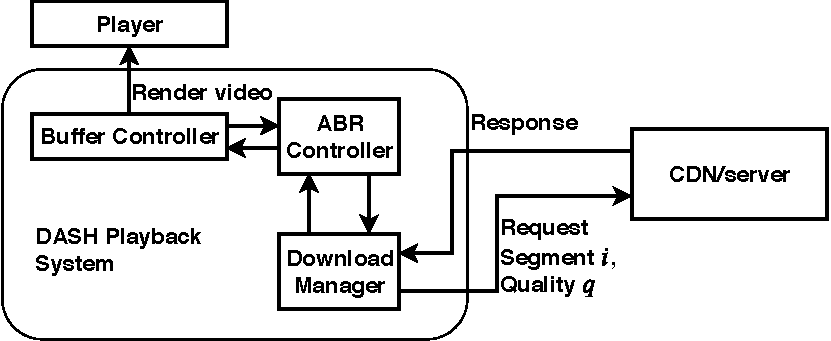
\includegraphics[width=0.7\linewidth]{img/playerDiagram_basic}
   \end{center}
   \caption{\label{fig:playerDiagram_basic} Original DASH based streaming system.}
\end{figure}

The inter-connection of the modules are depicted in the Fig.~\ref{fig:playerDiagram_basic}. Here, the ABR controller controls the playback via buffer controller while instructing download manager to download appropriate segment in the appropriate time. The ABR controller is the most important component. There are active research going on to improve ABR controller. As ABR controller is the part of the player, it need to be implemented in client application it self. In case HTML based player, ABRs need to be implemented in javascript. The ABR algorithm like MPC\cite{dash:mpc}, BOLA\cite{dash:bola} or the algorithms described in \cite{dash:probe,dash:cs2p,dash:CFA,dash:rnb,dash:buffer} does not have any special library requirement and can be implemented easily in any technology. However, as machine learning based ABR algorithm like Pensieve\cite{dash:pensieve}, OBOE\cite{dash:oboe} or HotDASH\cite{dash:hotdash} need specialized machine learning (ML) library and very hard to implement if the technology does not have support for required library. So, it is very difficult to deploy these algorithm in browser based video player.

\begin{figure}[ht]
	\begin{center}
		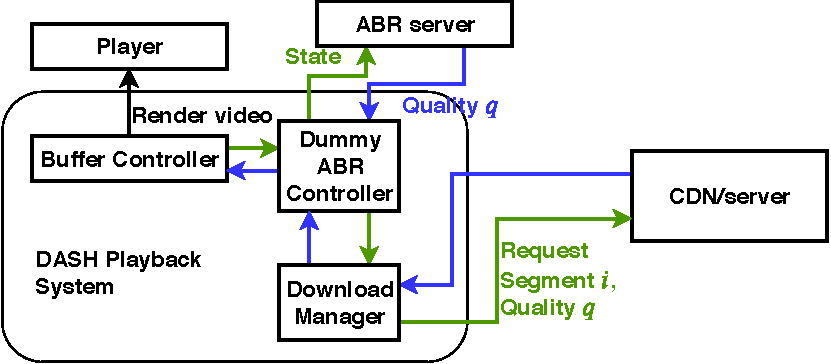
\includegraphics[width=0.7\linewidth]{img/playerDiagram_ml}
	\end{center}
	\caption{\label{fig:playerDiagram_ml} Modified DASH based streaming system to support ML based ABR algorithm}
\end{figure}

Authors of the ML based algorithm show prototype by modifying the system little bit. The new dash based video system looks like Fig.~\ref{fig:playerDiagram_ml}. Here they propose to replace the ABR controller in the client with a dummy one and run a ABR server in the local system. Every time, the player need to take a decision, dummy ABR controller contact ABR server with the current state of the player. The ABR server response the decision based on the algorithm of its choice.

The advantage of this system is that it does not depends on the client technology. ABR server can be implemented in any technology it suit best. However, it involves a extra communication with a external server which may be fatal to the viewing experience if the round trip time between the player and the ABR server. To avoid the communication delay between the player and ABR server, the ABR server need to run in local system only. This system is not easy to deploy as it need to a ABR server of each and every player.

\subsection{Split-DASH architecture}
\label{sec:Split_DASH_architecture}
To solve above problem we propose Split-DASH architecture. In split-DASH architecture, we split the original DASH architecture into two parts, i) a dumb player or client and ii) a smart server side. The proposed architecture depicted in the Fig.~\ref{fig:playerDiagram_split}.
\begin{figure}[ht]
	\begin{center}
		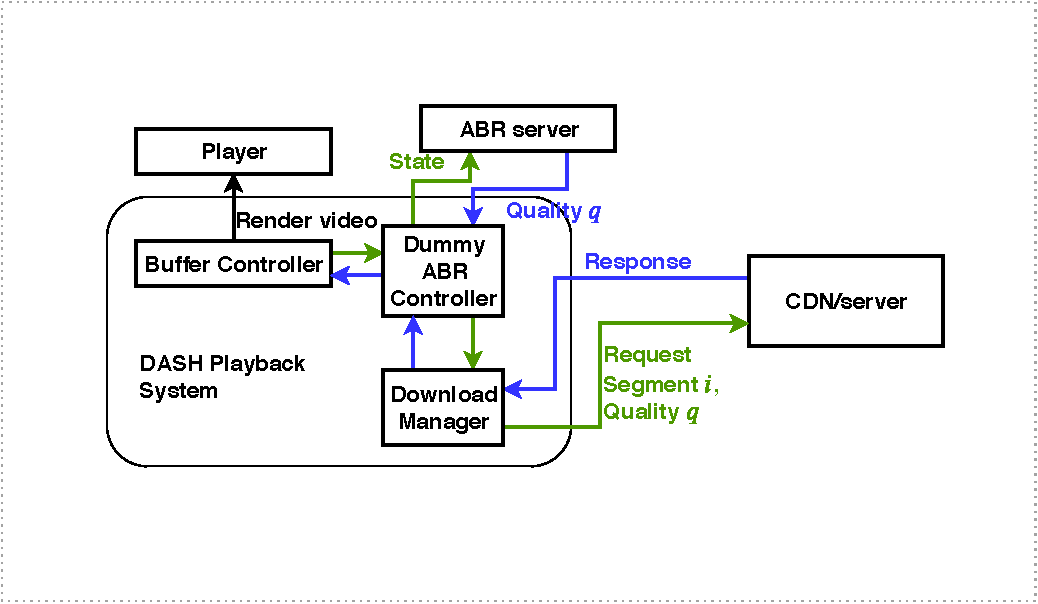
\includegraphics[width=0.9\linewidth]{img/playerDiagram_split}
	\end{center}
	\caption{\label{fig:playerDiagram_split} Modified DASH based streaming system to support ML based ABR algorithm}
\end{figure}
Here we make the player dumb. It controls the play back but it do not take any decision. Instead it depends on the decision provided by the smart part counter part in the server. The server provides the following decision: i) time to download a segment, and ii) quality of the segment. Before we explain functionality of different modules in the server and client, we explain the transaction between dumb-client and the smart server. 

\begin{figure}[h]
	\begin{center}
		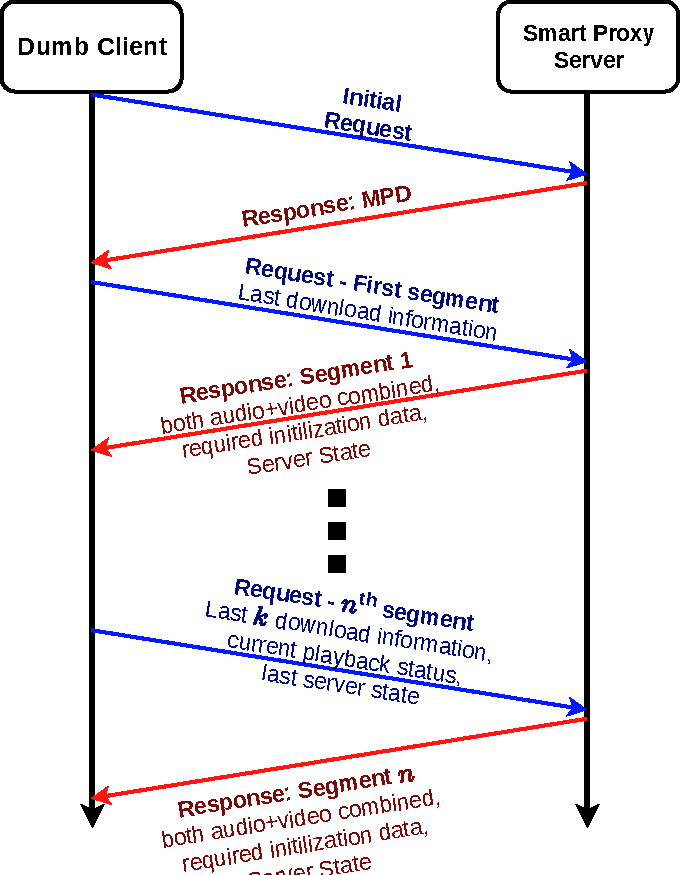
\includegraphics[width=0.5\linewidth]{img/splitDASHTransaction}
	\end{center}
	\caption{\label{fig:splitDASHTransaction} Modified DASH based streaming system to support ML based ABR algorithm}
\end{figure}

The Fig.~\ref{fig:splitDASHTransaction} depict the transaction between smart proxy server and dumb client. At first client request the Media Presentation Description (MPD) from the server. The smart proxy server returns a un-modified MPD for the video. However, it also adds a server identifier {\tt X-Server-Type: Smart}. This identifier indicate that the server is not simple CDN server, instead, it is a smart proxy server. So, the dumb client prepare the HTML video element and request for the first video segment. Here client does not mention the video/audio quality for the segment. Instead, client enclose the download history with the request. When the server receives a request, it looks for old server state in the request. If present, it will expand the state, other wise, it create a new state. Then, update the state according to the current playback information and download history provided in the request. Based on this information, server calculate the best quality for both audio and video segment based on the pre-decided ABR algorithm. Once quality is decided, it download the required segments of the calculated quality from the CDN/streaming (if not available in it cache) and send it back to the dumb player. It Also calculate the time player should wait (i.e. sleep time) before sending another request to the server. It multiplexes the sleep time and server state with the request. The contents of the server state is dependent of the ABR algorithm. Most of the deterministic ABR algorithm, does not required to maintain any state, however, ABR algorithm like pensieve need to maintain state. In case of pensieve, server state contains only the pensieve state.
Here we send server state to client to make server stateless. The client does not read the server state, however, it store it and send with next request.

\noteam{need to add overhead with a table or plot}


\section{SpEnDASH Architecture}
Recently we have developed a energy aware DASH based ABR algorithm EnDASH for smartphones. The algorithm is described in \noteam{cite/ref algo here}. The EnDASH algorithm heavily dependent on smartphone sensor data and neural-network driven ABR algorithm. We implement the EnDASH by modifying Split-DASH architecture (\ref{sec:Split_DASH_architecture}). We call it SpEnDASH architecture. The SpEnDASH architecture have 3 parts, i) A android application, ii) Modified split-DASH dumb client and iii) EnDASH aware smart proxy server. Fig.~\ref{fig:playerDiagram_SpEnDASH} describe the different components and interactions between those components. In this model, entire video playback system run inside a webview in an android application. The application collect several informations regarding the device and feed to the webview. The dumb player running inside the webview collect those data and send them to the server with the segment request. The server store those use all the informations to find out the next video quality using the EnDASH algorithm and return the response accordingly.
\begin{figure}[h!]
	\begin{center}
		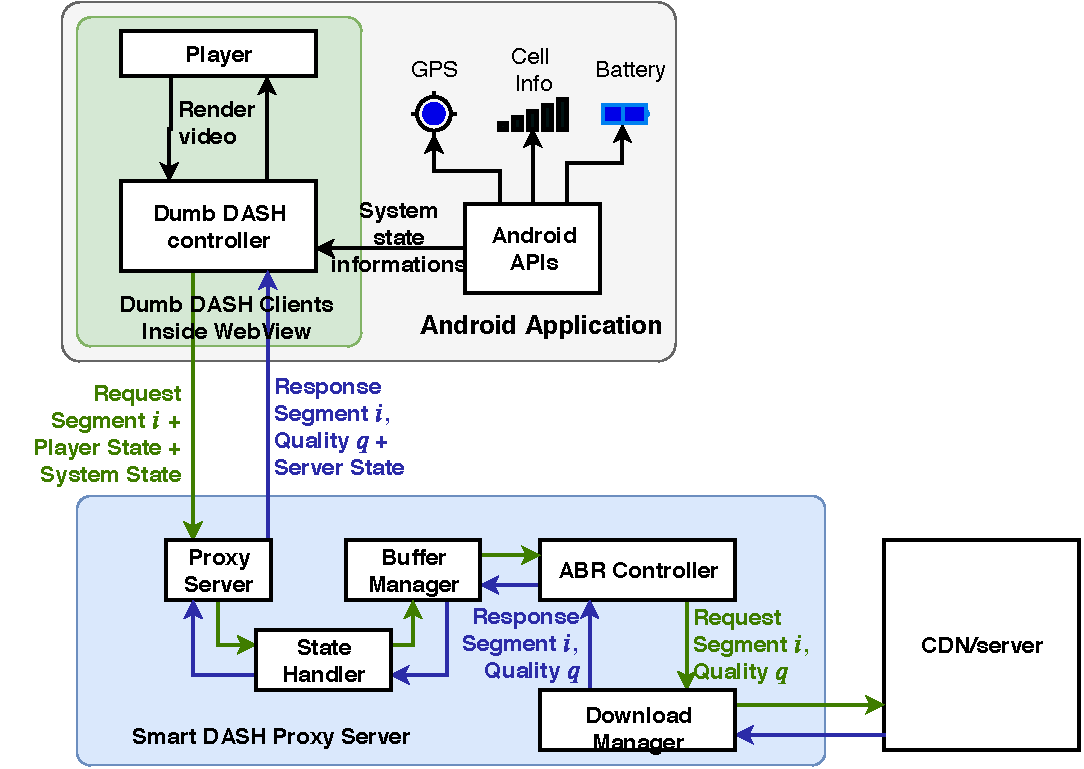
\includegraphics[width=0.9\linewidth]{img/playerDiagram_SpEnDASH}
%		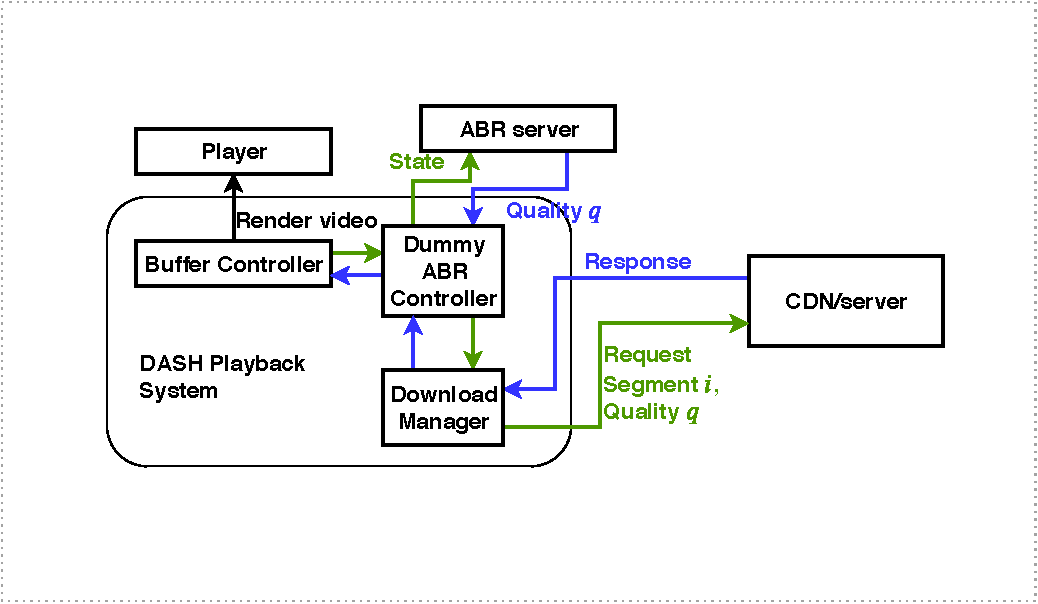
\includegraphics[width=0.9\linewidth]{img/playerDiagram_split}
	\end{center}
	\caption{\label{fig:playerDiagram_SpEnDASH} Modified DASH based streaming system to support ML based ABR algorithm}
\end{figure}

{\bf Advantages:}
%%
%\newcommand{\html}{{\tt HTML5 }}
\newcommand{\js}{{\tt JavaScript }}
\newcommand{\python}{{\tt Python }}


\section{Implementation}
We have describe the system architecture of Split-DASH architecture int he Section~\ref{sec:Split_DASH_architecture}. The architecture mainly have two parts, i) the dumb client and ii) the smart server. We choose \html and {\tt JavaScript} to implement the dumb client and \python based implementation for the smart server. Here the implementation details:

\subsection{The client}
We use the MSE of \html to implement the player which is being controlled by \js using Source Buffer API. This API allow us to add media segment and change the quality on the fly. MSE and \js is available in almost all the browser, so the client can in every device with \js and \html support.

In the client, \js contact the the smart server using AJAX call and get instruction. Our module also uses keep the track of ongoing AJAX call and abort the connect if the connection stay unresponsive for a threshold duration and restart the call again. This mechanism makes the client robust and network failure tolerant. The client plays video flawlessly unless the network is down for a long time.

\subsection{The server}
The smart server is a HTTP server with few extra capabilities mentioned in the Section~\ref{sec:Split_DASH_architecture}. In our implementation, there are three modules, i) the HTTP server, ii) the dummy client iii) the ABRs.

{\bf The HTTP server} module is the front end of the smart server. We implement it by extending \python {\tt BaseHTTPServer} module. As the \python does not support true multi-threading, we create new process as soon as the server receives a request and process the request in the newly created process.

The server create a new instance of dummy client and load the state from the request if available. The server pass the request to the dummy client to process it and wait to receive an action from it. The actions are mostly for the dumb client only. So it create the response the send the response to the server and end the process. However, if the response needs media segment, this module download those segments and pass those segments one after another in the body of the response.

{\bf the dummy client} instance represent the client state in the server. Upon receiving a request it update its state and consult the ABR for the quality for next segment. Once ABR decides the quality for next segment, it create the actions which includes the sleeping time and segments and qualities.

{\bf The ABRs} are the most important part of our module. In our implementation, ABRs are implemented independently from other modules. There is only one single entry point to a ABR from the dummy client module. This architecture provides a greate flexibility in ABR implementation. We implement the BOLA, and MPC as simple \python module and the pensive as different process and connect using a local socket API.



%%
%\section{Evaluation}
To evaluate our proposed streaming system, we compare \textit{CoaliDASH} with existing streaming systems and adaptation algorithms. Apart from \textit{CoaliDASH}, we have implemented two different streaming systems under the environment module --  {\it Simple} and {\it DHT based}. The {\it Simple} environment emulates the DASH based client-server adaptive streaming where we have used three baselines -- BOLA~\cite{bola2-acm-mmsys2018}, MPC~\cite{MPC-SIGCOMM-2015} and Pensieve~\cite{Pensieve}.  The {\it DHT} environment represents an environment with a distributed hash table based peer-to-peer system \cite{ChordStoica,dht1}.
%\notesc{Give a citation for DHT.} 
All the above streaming clients have been implemented in Python\footnote{The source code of the implementation is available publicly at the following link -- \url{https://github.com/abhimp/CoaliDASH}} and has been executed over an emulation environment as discussed next. 
%Our proposed algorithm is based on collaborative segment downloading. It important to have a large set of players in the network, otherwise it falls back as a standalone player with BOLA as the ABR. It is difficult to have such a big network in a real environment, and it is more difficult to configure such a big network with different network condition. To avoid all these issues, we emulate the streaming player on top of a simulated environment.

\subsection{Emulation Environment}
\label{sec:simulatorprop}
We develop a emulator platform similar to~\cite{Pensieve} to analyze the performance of \textit{CoaliDASH} under diverse environments. The developed emulation environment has the following features. All the players in the system have access to system clock which is an event-driven clock handled by the emulator core. The emulator uses a reference network to define the connectivity across the networked nodes; where every node of the network runs a streaming player. The network characteristics (bandwidth, delay between two nodes) of the reference network has been used to configure the network characteristics of the emulated network. We maintain a global playback time; the streaming server does not reveal any informations about a segment unless that segment can be downloaded according to the global playback time. We use Mahimahi \cite{mahimahi} network traces to emulate the network condition of the links between video server to a player, based on the reference network. We have randomly assigned different Mahimahi traces to every player in a network. The emulated player can use any existing ABR implementation without any modification as long as it takes the player-state as the input and gives the next segment quality as the output. 
%	\item The simulator can emulate a network if it runs with a reference network. It places a player per node of the reference network.
%	\item Any Two players in the system communicate only through the emulated network. For the emulated network, simulator needs a reference network which will provide the bandwidth delay between two nodes. We calculate communication delay carefully and a conservative way so that it does not violets the real communications between delay. For TCP like communication between two play in the simulated network, we calculate the transmission time based the delay and sender buffer. It is not accurate, but it gives higher transmission time than our empirical studies.
%	\item A player will never access the future video information. We maintain a global playback time. The video server module will never reveal any informations about a segment unless that segment can be downloaded according to the global playback time.
%	\item We use Mahimahi \cite{mahimahi} like network trace to simulate the network condition of the links between video server to a player. We randomly assigned different Mahimahi traces to every player in a network.
%	\item The emulated player can use any existing ABR implementation without any modification as long as it takes the player state as input and gives next segment quality as the output. This feature eliminates the possibility of faulty implementation.
%\end{itemize}
In the emulated environment, we use Eq.~(\ref{eqn:transmissionTime}) to compute the transmission time $T_{ij}$ between two players $P_i$ and $P_j$ in a coalition. Here $clen$ is the data length of the video segment, $d_{ij}$ is delay between two nodes, $buf$ is the sender buffer and $x$ is the noise factor which is uniformly distributed between $\theta_1$ to $\theta_2$. 
%\notesc{What is $P(x)$?}
\begin{align}
T_{ij} = clen\times \frac{buf}{2\times d_{ij}} \times x \mbox{\hspace{1cm}}& \theta_1 <= x <= \theta_2  
%& \mathcal{p}(x) = \frac{1}{\theta_2 - \theta_1} 
\label{eqn:transmissionTime}
\end{align}



%
%\begin{figure}[ht]
%	\captionsetup[subfigure]{}
%	\begin{center}
%		\subfloat[\label{fig:avgBitratebox} Averge Bitrate]{
%			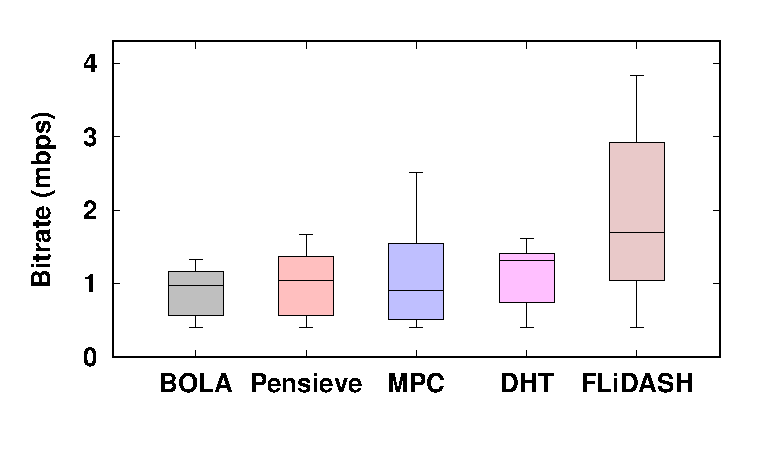
\includegraphics[width=0.49\linewidth]{img/grpbasic/avgbitrate_box_1}
%		}
%		\subfloat[\label{fig:avgBitratecmf}Average Bitrate]{
%			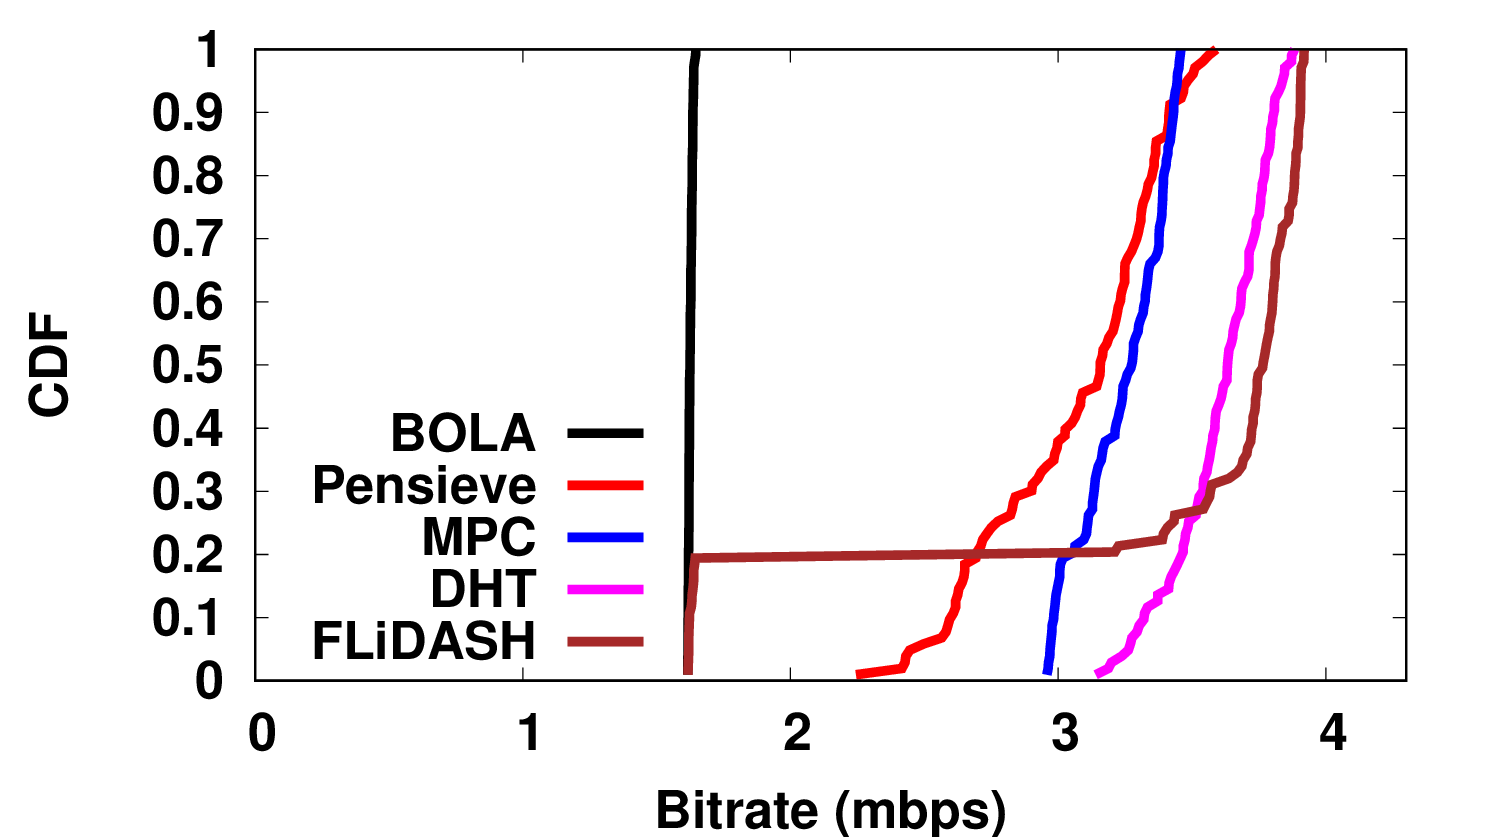
\includegraphics[width=0.49\linewidth]{img/grpbasic/avgbitrate_cdf_1}
%		}
%	\end{center}
%	\caption{\label{fig:avgBitrate} Average bitrate played}
%\end{figure}



%\begin{figure}[ht]
%	\captionsetup[subfigure]{}
%	\begin{center}
%		\subfloat[\label{fig:avgBitrateVarbox}]{
%			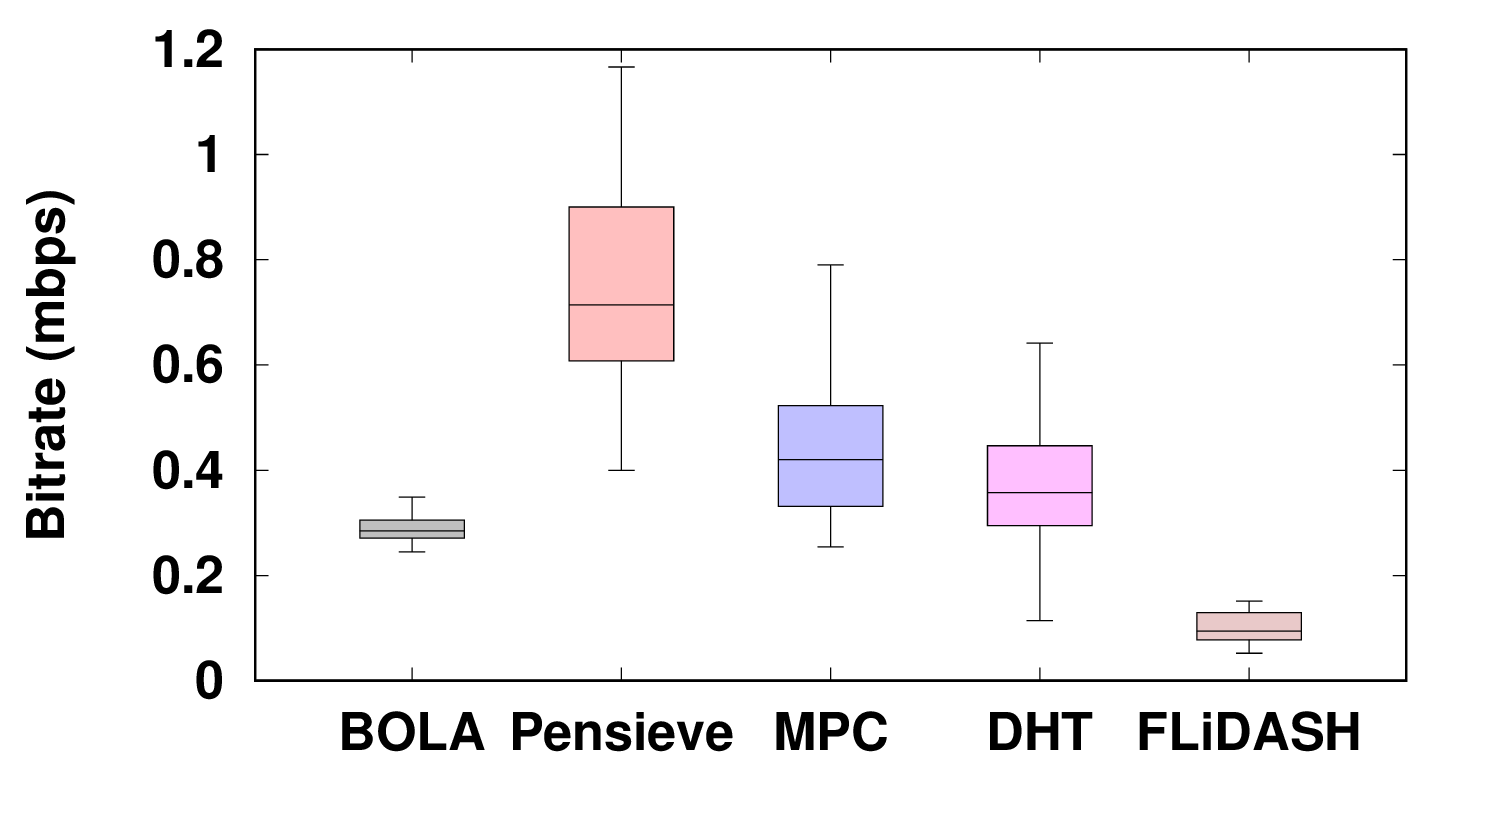
\includegraphics[width=0.49\linewidth]{img/grpbasic/avgbitrate_var_box_1}
%		}
%		\subfloat[\label{fig:avgBitrateVarcmf}]{
%			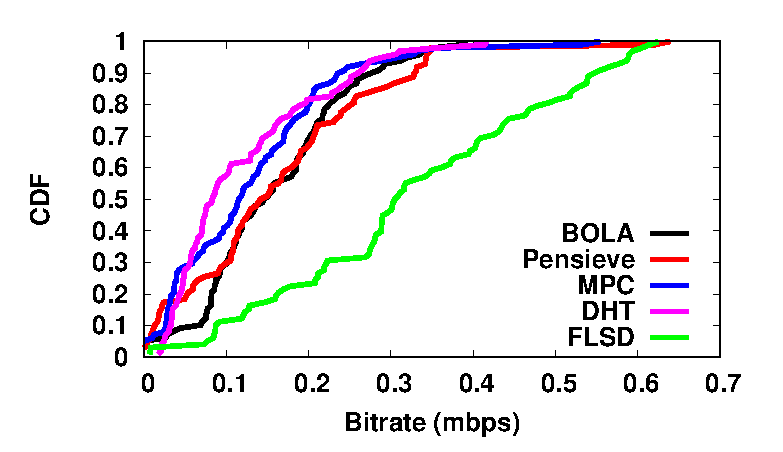
\includegraphics[width=0.49\linewidth]{img/grpbasic/avgbitrate_var_cdf_1}
%		}
%	\end{center}
%	\caption{\label{fig:avgBitrateVar} Average bitrate variation during playback}
%\end{figure}




%As we discussed at \ref{sec:simulatorprop}, we designed all this environment carefully so that it emulates real network condition and does not take any unfair advantage of the fact that everything is directly accessible. We use BOLA as the base ABR for every environment if not specified otherwise. We compared our system with BOLA, MPC and Pensieve ABR. We use the implementation provided by Pensieve source code directly for BOLA, MPC and Pensieve. The {\it Simple} environment was used as the environment while experimenting with BOLA, MPC and Pensieve. Although we run experiments with both RobustMPC, we have shown only RobustMPC results of RobustMPC as results are almost the same. As BOLA, MPC and Pensieve are ABR for the single player streaming system, we implement DHT as a baseline of the peer-to-peer system.

\subsection{Experimental Setup}
We run our emulation with a large set of autonomous system data available from SNAP database~\cite{ASDataSet} as reference networks. We have executed the systems over 710 reference networks, with 100 to 1000 nodes per network. As mentioned earlier, every network node runs a streaming client. To train the model for learning based adaptive streaming like Pensieve~\cite{Pensieve}, we use $58$ DASH-ified videos with a total duration of $45$ hours. We have taken only lengthy videos for our experiment because most of the live online live streaming lasts more than one hour \cite{LiveStreamDuration1,LiveStreamDuration2}. We have created Mahimahi compatible traces from publicly available dataset, like a broadband trace from FCC~\cite{dataset-fcc} and the 3G/HSDPA mobile dataset collected in Norway~\cite{dataset-norway}. We modified these datasets as described in \cite{Pensieve} to make it Mahimahi compatible.

For experimentation, we use the QoE definition as given in \cite{Pensieve}. According to this definition, we consider three QoE components -- (i) average quality level, (ii) average jump in the quality level (smoothness of the video playback) and (iii) re-buffering time. Let $\mathcal{Q}_n$ denote the quality level for video segment $n$ and $\mathcal{T}_n$ be the re-buffering time. Considering that there are $N$ number of segments in a reference video, the average QoE is defined as follows. 
\begin{equation}
QoE = \frac{\alpha}{N}\sum_{n=0}^{N} \mathcal{F}(\mathcal{Q}_n) - \frac{\beta}{N-1} \sum_{n=1}^{N}\lvert\mathcal{F}(\mathcal{Q}_n) -\mathcal{F}(\mathcal{Q}_{n-1})\rvert - \gamma\mathcal{T}_n
\label{eqn:QoE}
\end{equation}
Here, $\alpha$, $\beta$ and $\gamma$ are weight factors (values between 0 and 1) to individual components, such that $\alpha + \beta + \gamma = 1$. 


%\begin{figure}[h]
%	\captionsetup[subfigure]{}
%	\begin{center}
%		\subfloat[\label{fig:Stall_Timebox}]{
%			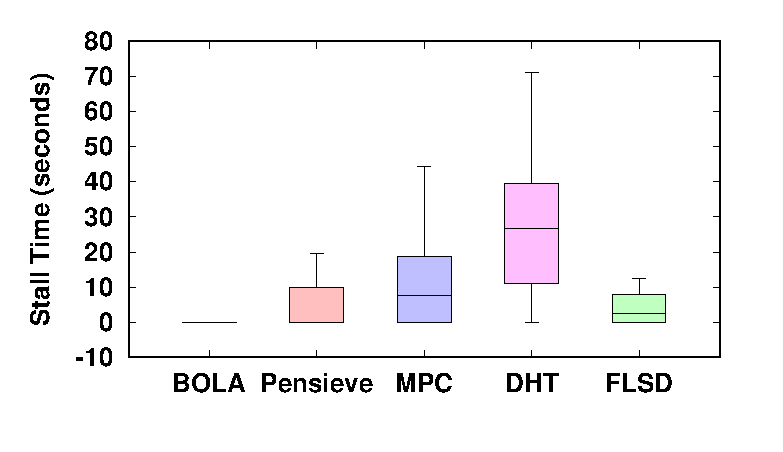
\includegraphics[width=0.49\linewidth]{img/grpbasic/stalltime_box_1}
%		}
%		\subfloat[\label{fig:Stall_Timecmf}]{
%			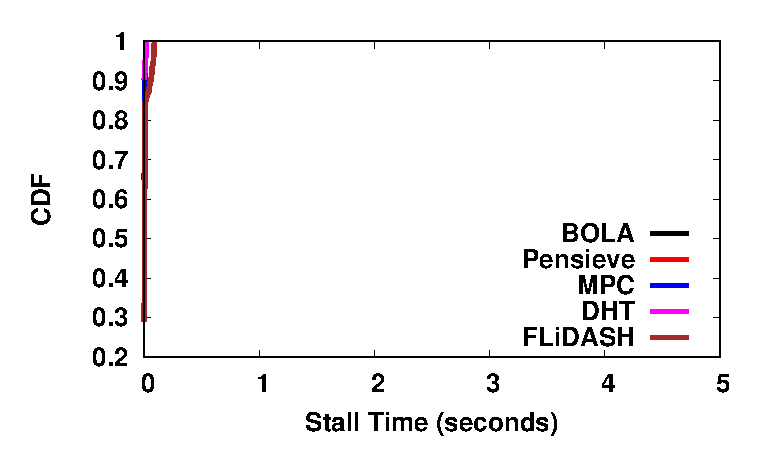
\includegraphics[width=0.49\linewidth]{img/grpbasic/stalltime_cdf_1}
%		}
%	\end{center}
%	\caption{\label{fig:Stall_Time}Total stall time observed each player}
%\end{figure}
%
%\begin{figure}[h]
%	\captionsetup[subfigure]{}
%	\begin{center}
%		\subfloat[\label{fig:QoEbox}]{
%			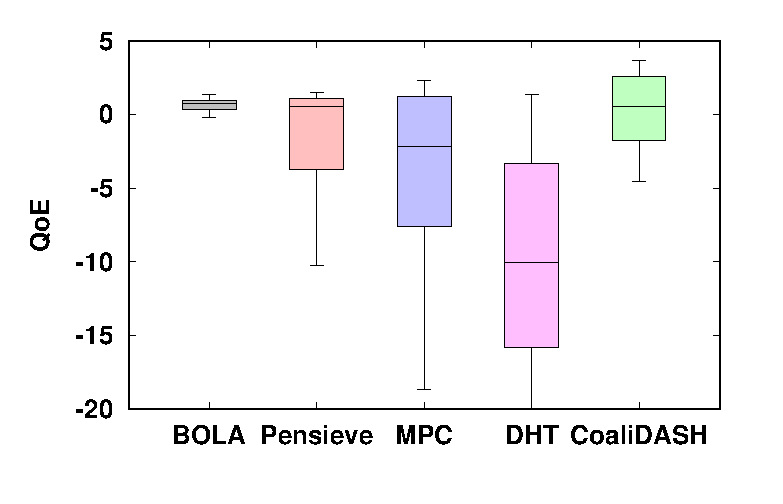
\includegraphics[width=0.49\linewidth]{img/grpbasic/qoe_box_1}
%		}
%		\subfloat[\label{fig:QoEcmf}]{
%			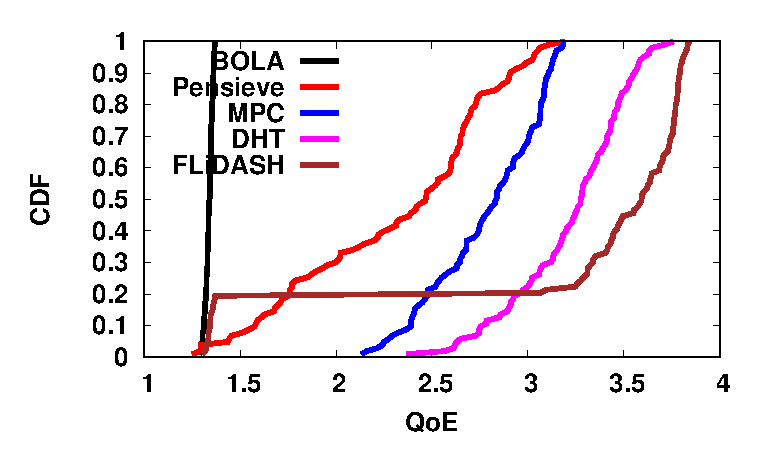
\includegraphics[width=0.49\linewidth]{img/grpbasic/qoe_cdf_1}
%		}
%	\end{center}
%	\caption{\label{fig:QoE}Quality of experience (linear)}
%\end{figure}


\begin{figure}[ht]
	\captionsetup[subfigure]{}
	\begin{center}
		\subfloat[\label{fig:avgBitratecmf}Average Bitrate]{
			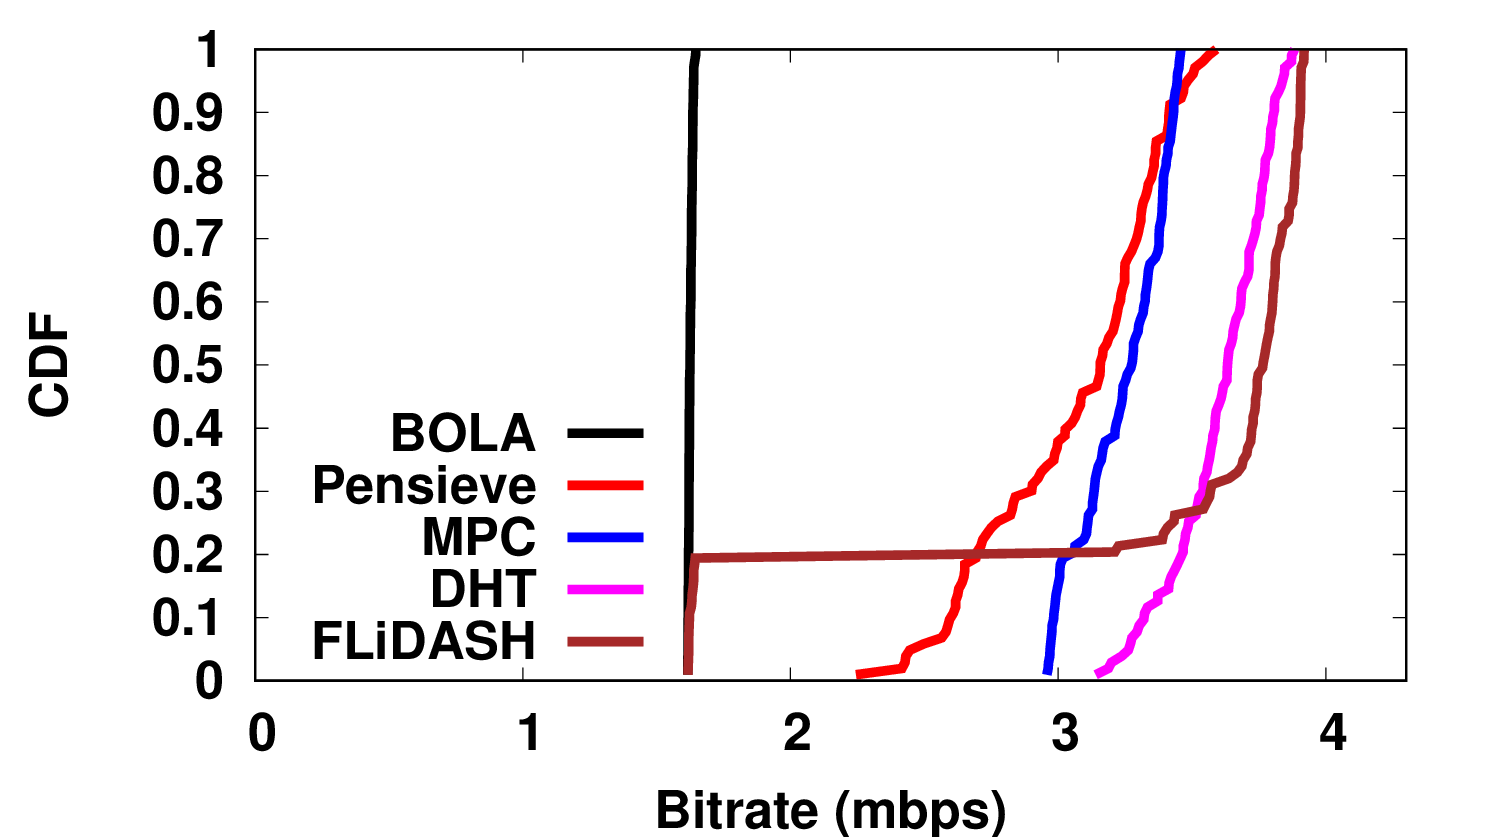
\includegraphics[width=0.49\linewidth]{img/grpbasic/avgbitrate_cdf_1}
		}
     	\subfloat[\label{fig:avgBitrateVarcmf}Bitrate Variation]{
     			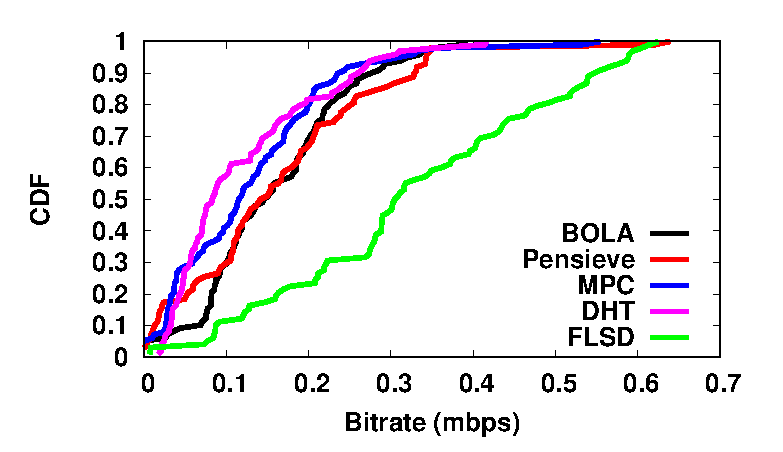
\includegraphics[width=0.49\linewidth]{img/grpbasic/avgbitrate_var_cdf_1}
     		}
	\end{center}
	\caption{\label{fig:avgBitrate} QoE Components: Average Bitrate and Bitrate Variation}
\end{figure}

\subsection{Results}
We first observe the individual QoE components for \textit{CoaliDASH} in comparison with other baselines. Fig.~\ref{fig:avgBitratecmf} compares the average playback bit-rate for various streaming applications. In Fig.~\ref{fig:avgBitrateVarcmf}, we show the variation in average playback bit-rates, which indicate the smoothness of the video rendering. We observe that the performance of BOLA in terms of average playback bit-rate is very low, and most of the players played the videos in lower average quality compared to other baselines. BOLA is very conservative about the bitrate, whereas it is much concerned about the re-buffering time. Pensieve and MPC improve the video quality compared to BOLA by utilizing reinforcement learning and deep inspection, respectively. DHT is the first system which uses the knowledge of existing players in the network and form a peer-to-peer architecture for collectively download the videos. So, it improves the average video quality compared to client-server based ABR. However, CoaliDASH clusters the players based on their network conditions and render the videos keeping the coalition members in sync. In Fig.~\ref{fig:avgBitratecmf}, it is clear that there are clusters of players who play a video in almost equal quality levels. Although we observe that the average variation in the video quality is higher for CoaliDASH; however, it is because the deviation of video quality levels among various coalitions. A coalition where majority of the members have low network resources, the average quality of the video gets drop down. 
%A slight change in the quality incurs high variation.

\begin{figure}[!ht]
	\captionsetup[subfigure]{}
	\begin{center}
		\subfloat[\label{fig:Stall_Timecmf}Total Re-buffering Time]{
			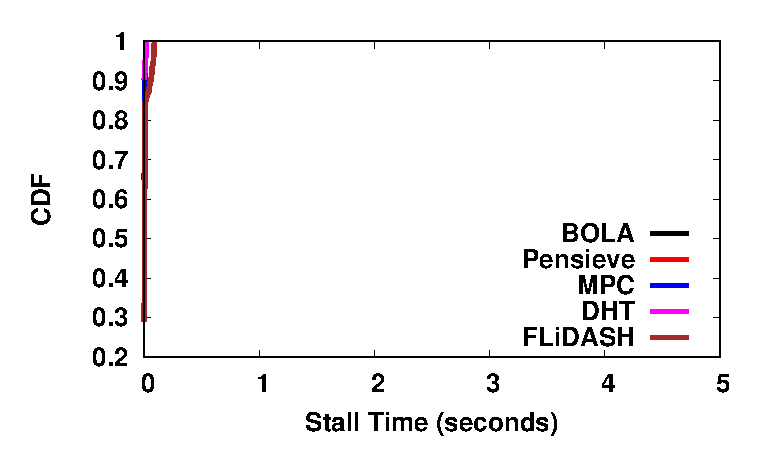
\includegraphics[width=0.49\linewidth]{img/grpbasic/stalltime_cdf_1}
		}
       	\subfloat[\label{fig:QoEcmf}Overall QoE]{
       			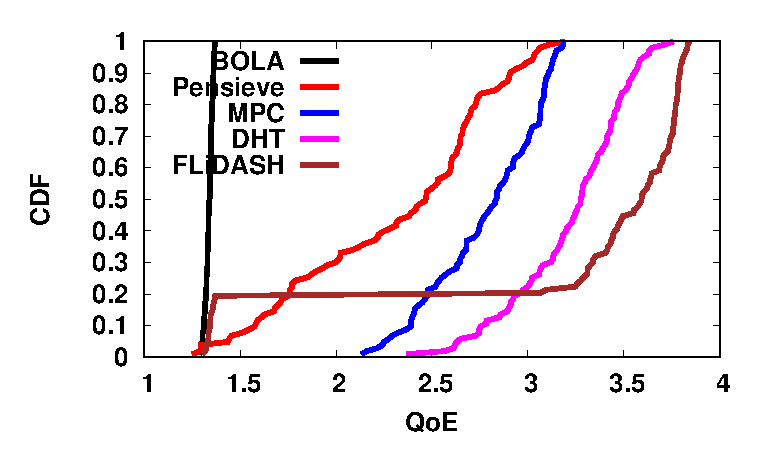
\includegraphics[width=0.49\linewidth]{img/grpbasic/qoe_cdf_1}
       		}
	\end{center}
	\caption{\label{fig:avgBitrateVar} Re-buffering Time and Overall QoE}
\end{figure}

Next, Fig.~\ref{fig:Stall_Timecmf} compares the total re-buffering time among various baselines. We observe that the re-buffering time is very high for DHT because it needs more time to search for a video segment from the network before it can fetch it directly from the streaming server. The re-buffering time for CoaliDASH is moderated although it includes the skip time during the synchronization among the members of the coalition. BOLA incurs almost no re-buffering time; whereas Pensieve and MPC suffer from noticeable re-buffering time. As the re-buffering time is a significant contributor in the overall QoE measurement (Eq.~(\ref{eqn:QoE})), the overall QoE for various baselines, as shown in Fig.~\ref{fig:QoEcmf}, indicates that \textit{CoaliDASH} outperforms other baselines in term of maximum achievable QoE.  Among the various scenarios simulated over our developed platform, more than $50\%$ of the cases, \textit{CoaliDASH} incurs a high QoE (value between $2$--$4$). 

\begin{figure}[!ht]
	\captionsetup[subfigure]{}
	\begin{center}
		\subfloat[\label{fig:cdnuploaded_byte} Data downloaded from the server]{
			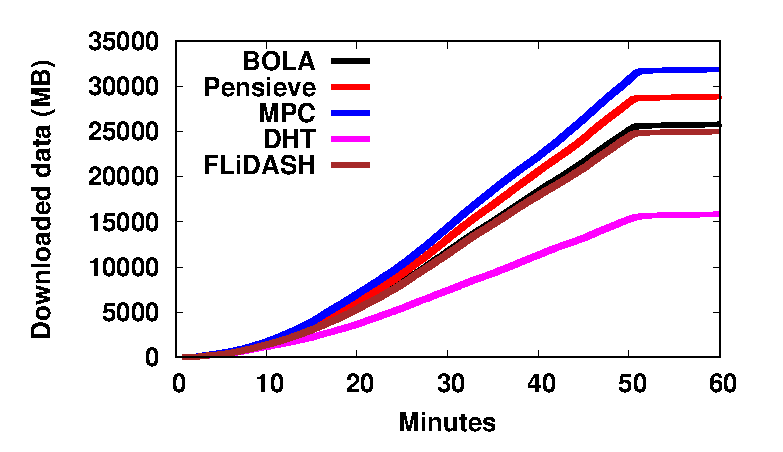
\includegraphics[width=0.49\linewidth]{img/grpbasic/cdnupload_1}
		}
		\subfloat[\label{fig:cdnuploaded_cnt} \# of segment downloads from the server]{
			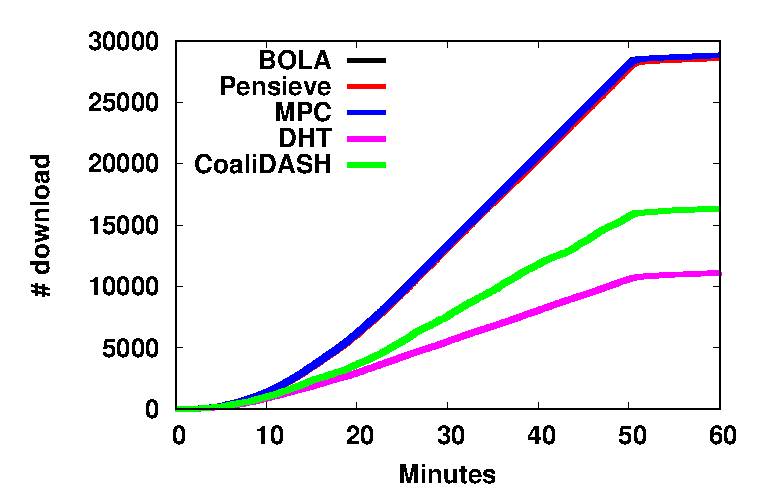
\includegraphics[width=0.49\linewidth]{img/grpbasic/cdnuploadcnt_1}
		}
	\end{center}
	\caption{\label{fig:cdnuploaded}Streaming Server Usages}
\end{figure}

One of the major objectives of \textit{CaliDASH} is to reduce the usage of streaming server when multiple co-located streaming players play the same live video. In Fig.~\ref{fig:cdnuploaded}, we plot the streaming server usage by different baselines in terms of the total bytes downloaded from the streaming server and the number of video segments directly downloaded from the streaming server. We observe that that the streaming server usages by DHT is lowest. In the case of CoaliDASH, players are bounded to receive data from its group only, while in case of DHT, a player can share segments with as many players as possible. The standalone players need to download all the segments directly from the server. Therefore, we observe a performance trade-off here -- \textit{CoaliDASH} significantly improves the QoE performance while having little increase in the streaming server load. In a nutshell, the proposed approach makes a balance between the QoE and streaming server load during the peer-assisted live video streaming.  


%Fig.~\ref{fig:avgBitrate}, \ref{fig:avgBitrateVar}, \ref{fig:Stall_Time} and \ref{fig:QoE} we report the general result we found from our experiment. Fig.~\ref{fig:QoE} is a plot of Quality of Experience. We calculate QoE using the Equation~\ref{eqn:QoE}. In the equation, $\alpha$ is the quality factor and $\beta$ and $\gamma$ are smoothness penalty and stall penalty.
%
%
%
%According to Fig.\ref{fig:avgBitrate} performance of BOLA very low and most of the players played in lower quality. BOLA is very conservative about the bitrate and very much concerned about the rebuffering time. Pensieve and MPC improved the video quality compared to the BOLA by utilising reinforcement learning and deep inspection respectively. DHT is the first system which uses the knowledge of existing players in the network. So, it improves an average video quality compared to ABR. However, CoaliDASH clustered the players and played video in sync. In Fig.~\ref{fig:avgBitratecmf}, it is clear that there are clusters of players who played video in almost equal quality. Average variation in video quality is higher for CoaliDASH. However, it is higher because it played in the video in high quality. A slight change in the quality incurs high variation.


%\begin{figure}[h]
%\captionsetup[subfigure]{}
%\begin{center}
%	\subfloat[\label{fig:benfit_bitrate} Benefit in terms of average bitrate]{
%		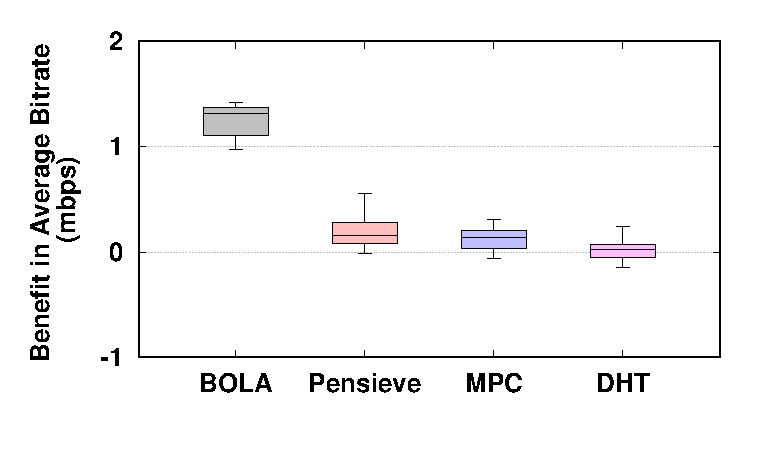
\includegraphics[width=0.49\linewidth]{img/grpbasic/benefit_bitrate_box_1}
%	}
%	\subfloat[\label{fig:benefit_qoe} Benefit in terms of QoE]{
%		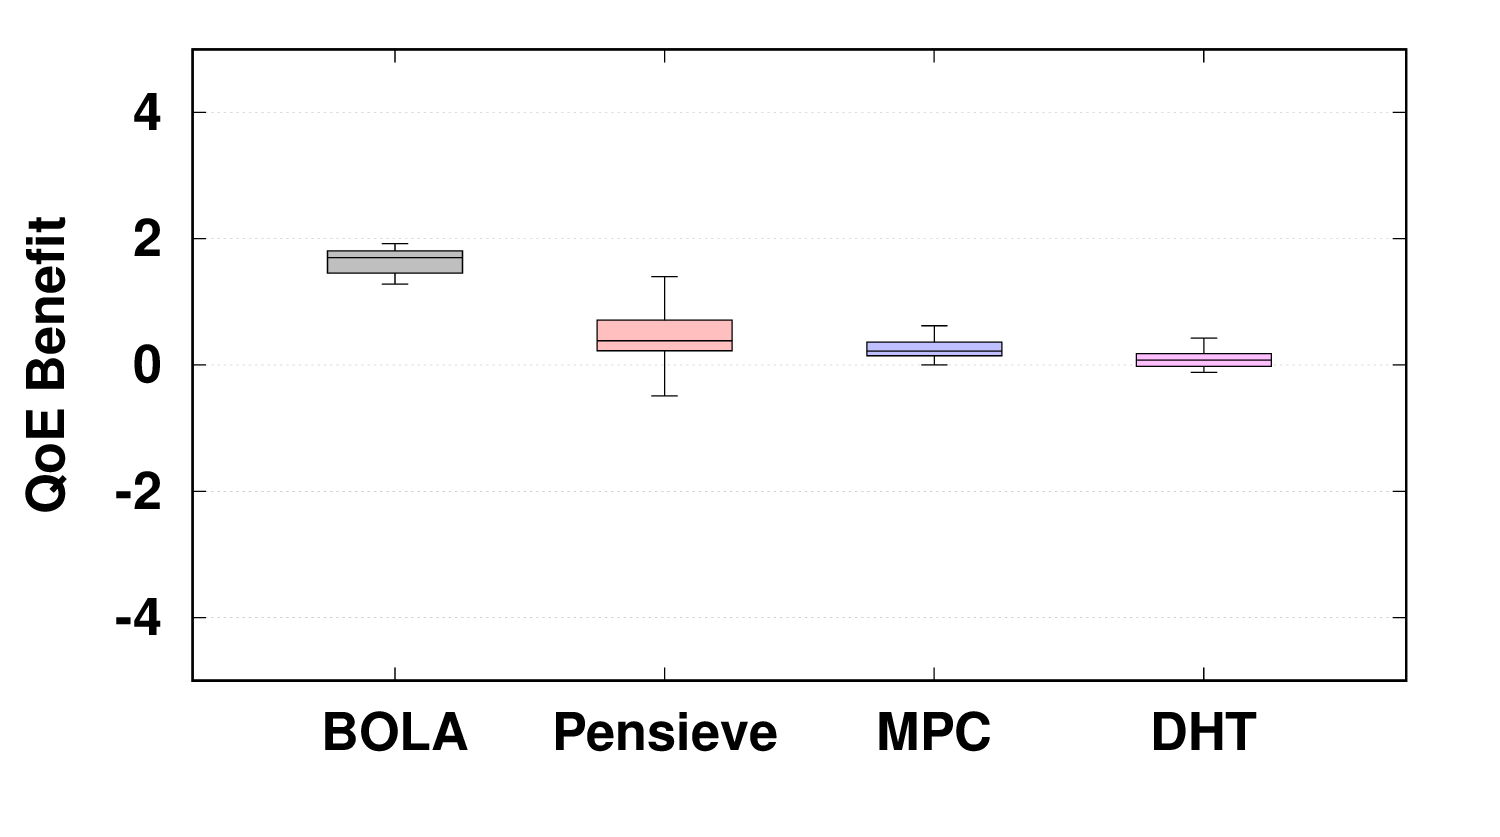
\includegraphics[width=0.49\linewidth]{img/grpbasic/benefit_qoe_box_1}
%	}
%\end{center}
%\caption{\label{fig:benefit}Per player benefit of using CoaliDASH}
%\end{figure}



\begin{figure*}[h]
	\captionsetup[subfigure]{}
	\begin{center}
		\subfloat[\label{fig:grp_qoe}Overall QoE]{
			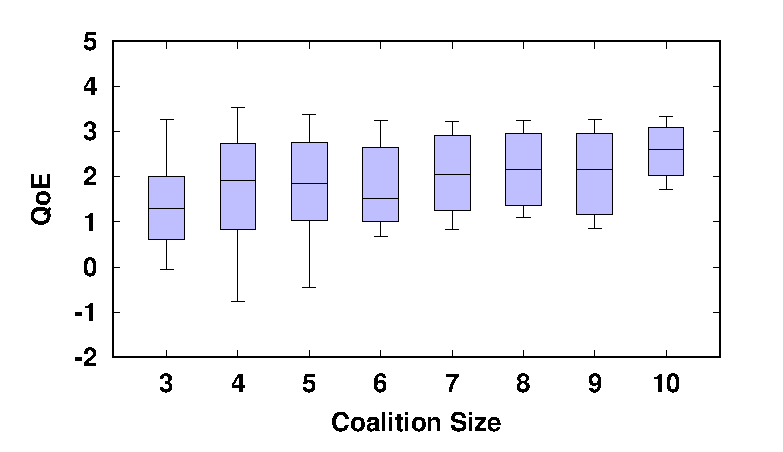
\includegraphics[width=0.33\linewidth]{img/grpbasic/grpsz_qoe}
		}
		\subfloat[\label{fig:grp_download}Amount of Data Upload and Download]{
			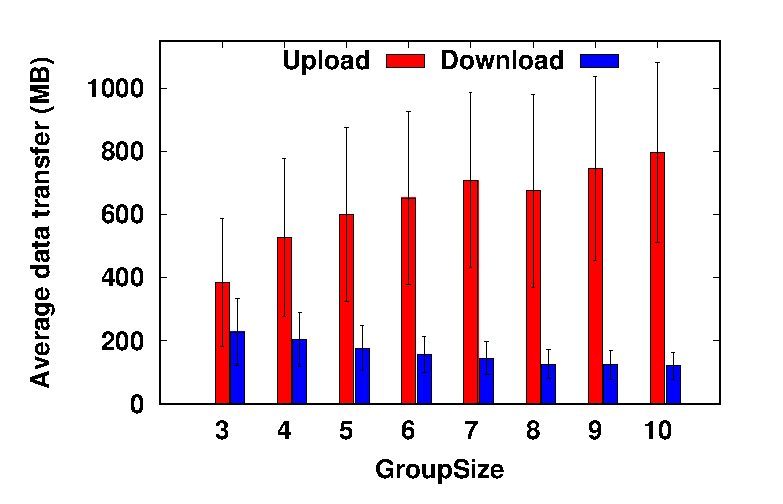
\includegraphics[width=0.33\linewidth]{img/grpbasic/grpsz_upload_download}
		}
       	\subfloat[\label{fig:grp_fairness}Fairness]{
       			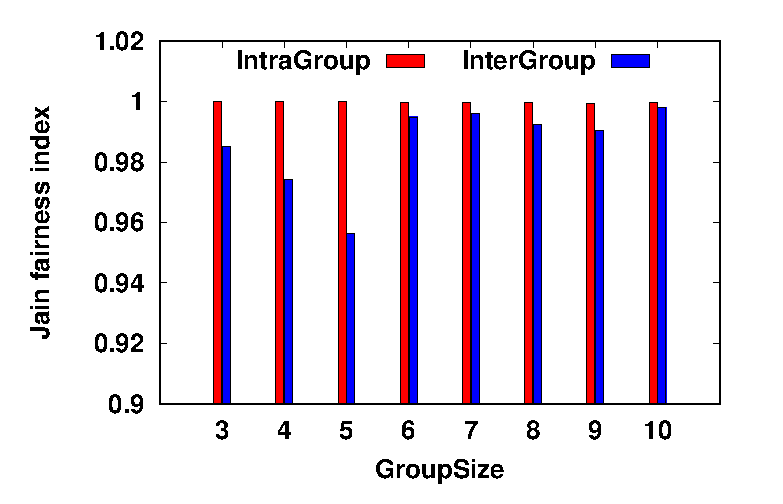
\includegraphics[width=0.33\linewidth]{img/grpbasic/grpsz_fairness}
       		}
	\end{center}
	\caption{\label{fig:grpsz}Effect of Coalition Size}
\end{figure*}





%\subsection{Benefit of using CoaliDASH}
%In Fig.~\ref{fig:benefit}, we report the benefit of using CoaliDASH instead of another streaming system for each player in the system. Here we plot only two metrics, i.e. average bitrate and QoE. To measure the benefit of using CoaliDASH we need to keep the environment (i.e. network condition) of a player same for each ABR and reference network. It is possible for because our environment is simulated and the entire simulation state depends on the initial random variable\footnote{We use pseudo-random variable available in {\tt python numpy} library. It generates the same sequence of random numbers for the same seed/initial state.} state. However, it means that every time we run the experiment with the same environment, ABR and reference network, we get the same result. For this reason, we do not run the same experiment with the same environment, ABR and network. However, to measure the benefit of using CoaliDASH instead of other ABR, we run an experiment on a large set of environments and reference network. We use Equation~\ref{eqn:benefit} to compute the benefit of a single player. Here $G_g$ is the metric for using CoaliDASH and $G_o$ is the same metric for other ABR. We plot all the benefit as a box plot. Here benefit $Ben(S)==0$ means CoaliDASH performed precisely the same as the other ABR. The positive and negative benefit means the better or worse performance of CoaliDASH compared to other ABR.
%\begin{equation}
%Ben(S) = \frac{G_g - G_o}{|G_o|}
%\label{eqn:benefit}
%\end{equation}
%From Fig.~\ref{fig:benefit}, we can see that most of the player in the experiments gain some forms of benefit in terms of average playback quality as well as the QoE. The slight degradation in the benefit in terms of QoE with compared to BOLA. We have already seen in the Fig.\ref{fig:QoE} that QoE of BOLA is very high although the average quality is low because of its very low stall time. However, the overall performance of CoaliDASH is higher than any other existing ABR or systems.
%\subsection{Effect of group size}
In all the previous experiments, we have fixed the maximum coalition size to 4 players. Here we check the effect of the increasing the coalition size. Fig.~\ref{fig:grp_qoe} and Fig.~\ref{fig:grp_download} shows the impact of different coalition sizes on the overall QOE and the total amount of data downloaded from the streaming server, respectively. We observe that a large coalition size provides better QoE because it gives more time to download a segment. However, in the case of a large coalition, every player has to upload more data to the other members of the coalition, which incurs an additional overhead.

%\subsection{Fairness}
In collaborative scenario, fairness among the members is an important metric. In our evaluation, we measure the fairness among the coalition members using Jain fairness index on QoE among the players \cite{jain1999throughput}. We measure the fairness among players in two categories, i) intra-coalition fairness (fairness among the coalition members of a coalition) and ii)inter-coalition fairness (fairness among the coalitions). The results are reported in Fig.~\ref{fig:grp_fairness}. We have computed fairness for seven different coalition sizes. Here we observe that the intra-coalition fairness index is always close to 1, which indicates a perfect fairness. However, inter-coalition fairness is not very high. It is expected as different coalitions can play video in different video quality which has a major contribution to the overall QoE. 
%From this result, we can conclude that CoaliDASH is fair.

%
%\section{Conclusion}
\label{chap03sec:conclusion}

In this work, we studied the internal working of YouTube's bitrate adaptation algorithm, by identifying important parameters and exploring their roles.
We observed that YouTube adapts segment length in addition to quality level, a behavior not been reported earlier.
As an implication, we observed that data wastage for a playback session is significantly lower than estimated previously.
We further provided an analytical model, augmented with a machine learning based classifier, to predict data consumption in adavance for a video playback session.
As an immediate future direction, we would like to explore other important implications of segment length adaption for YouTube.


\singlespacing
\small
\bibliographystyle{IEEEtran}
\bibliography{ref/dash} 
%

\end{document}
